% interactapasample.tex
% v1.05 - August 2017

\documentclass[]{interact}

\usepackage[hyphens]{url}

\usepackage[nolist,nohyperlinks]{acronym}
\usepackage{epstopdf}% To incorporate .eps illustrations using PDFLaTeX, etc.
\usepackage[T1]{fontenc}
\usepackage{lipsum}
\usepackage{lmodern}
\usepackage[caption=false]{subfig}% Support for small, `sub' figures and tables
%\usepackage[nolists,tablesfirst]{endfloat}% To `separate' figures and tables from text if required
%\usepackage[doublespacing]{setspace}% To produce a `double spaced' document if required
%\setlength\parindent{24pt}% To increase paragraph indentation when line spacing is doubled
\usepackage{wrapfig}
\usepackage[natbibapa,nodoi]{apacite}% Citation support using apacite.sty. Commands using natbib.sty MUST be deactivated first!
\setlength\bibhang{12pt}% To set the indentation in the list of references using apacite.sty. Commands using natbib.sty MUST be deactivated first!
\renewcommand\bibliographytypesize{\fontsize{10}{12}\selectfont}% To set the list of references in 10 point font using apacite.sty. Commands using natbib.sty MUST be deactivated first!
\usepackage{siunitx}

\theoremstyle{plain}% Theorem-like structures provided by amsthm.sty
\newtheorem{theorem}{Theorem}[section]
\newtheorem{lemma}[theorem]{Lemma}
\newtheorem{corollary}[theorem]{Corollary}
\newtheorem{proposition}[theorem]{Proposition}

\theoremstyle{definition}
\newtheorem{definition}[theorem]{Definition}
\newtheorem{example}[theorem]{Example}

\theoremstyle{remark}
\newtheorem{remark}{Remark}
\newtheorem{notation}{Notation}

\acrodef{ALUM}[ALUM]{Australian Land Use and Management}
\acrodef{DGGS}[DGGS]{discrete global grid system}
\acrodef{GIS}[GIS]{geographic information system}
\acrodef{GISc}[GIScience]{geographic information science}
\acrodef{NLM}[NLM]{neutral landscape model}
\acrodef{OLAP}[OLAP]{online analytical processing}
\acrodef{RAT}[RAT]{raster attribute table}
\acrodef{SQL}[SQL]{structured query language}
\acrodef{SSIF}[SSIF]{Strategic Science Investment Fund}

% A graphical abstract may also be included if required. Within the \verb"abstract" environment you can include the code
% \begin{verbatim}
% \\\resizebox{25pc}{!}{\includegraphics{abstract.eps}}
% \end{verbatim}
% where the graphical abstract is to appear, where \verb"abstract.eps" is the name of the file containing the graphic (note that \verb"25pc" is the recommended maximum width, expressed in pica, for the graphical abstract in your manuscript).

\begin{document}

%TC:ignore
\articletype{ORIGINAL RESEARCH ARTICLE}% Specify the article type or omit as appropriate

\title{Using a \acl{DGGS} for a scalable, interoperable, and reproducible system of land-use mapping}

\author{
    \name{Richard M. Law\textsuperscript{a,b}\thanks{Corresponding Author: R.~M. Law. Email: lawr@landcareresearch.co.nz}
    and James Ardo\textsuperscript{a,c}}
    \affil{\textsuperscript{a}\footnotesize{Landcare Research, Private Bag 11052, Palmerston North, New Zealand}
    \\
    \textsuperscript{b}\footnotesize{\url{https://orcid.org/0000-0002-7400-2530}}
    \\
    \textsuperscript{c}\footnotesize{\url{https://orcid.org/0009-0008-1201-9733}}
}}

\maketitle
%TC:endignore

\begin{abstract}
An accurate and timely land-use map of an area is a valuable geospatial dataset. Making one requires assembling heterogeneous geospatial input data. This becomes computationally expensive as the number of inputs grow or the combinational classification logic becomes more convoluted. We present as a solution an analytical framework based on a \ac{DGGS}. This provides a spatial data structure that: facilitates horizontal scaling; improves geospatial data interoperability; and makes classified geospatial data easier to reproduce. We demonstrate a benchmark of land-use assignment with a \ac{DGGS} against the vector and raster geospatial data models. Significant performance benefits are apparent over the vector case, while performance is equivalent to raster. Yet a \ac{DGGS} has other compelling benefits that makes it more convenient to use in the domain of land-use assignment than the raster data model.
\end{abstract}

%TC:ignore

% Graphical abstract
% \begin{center}
% 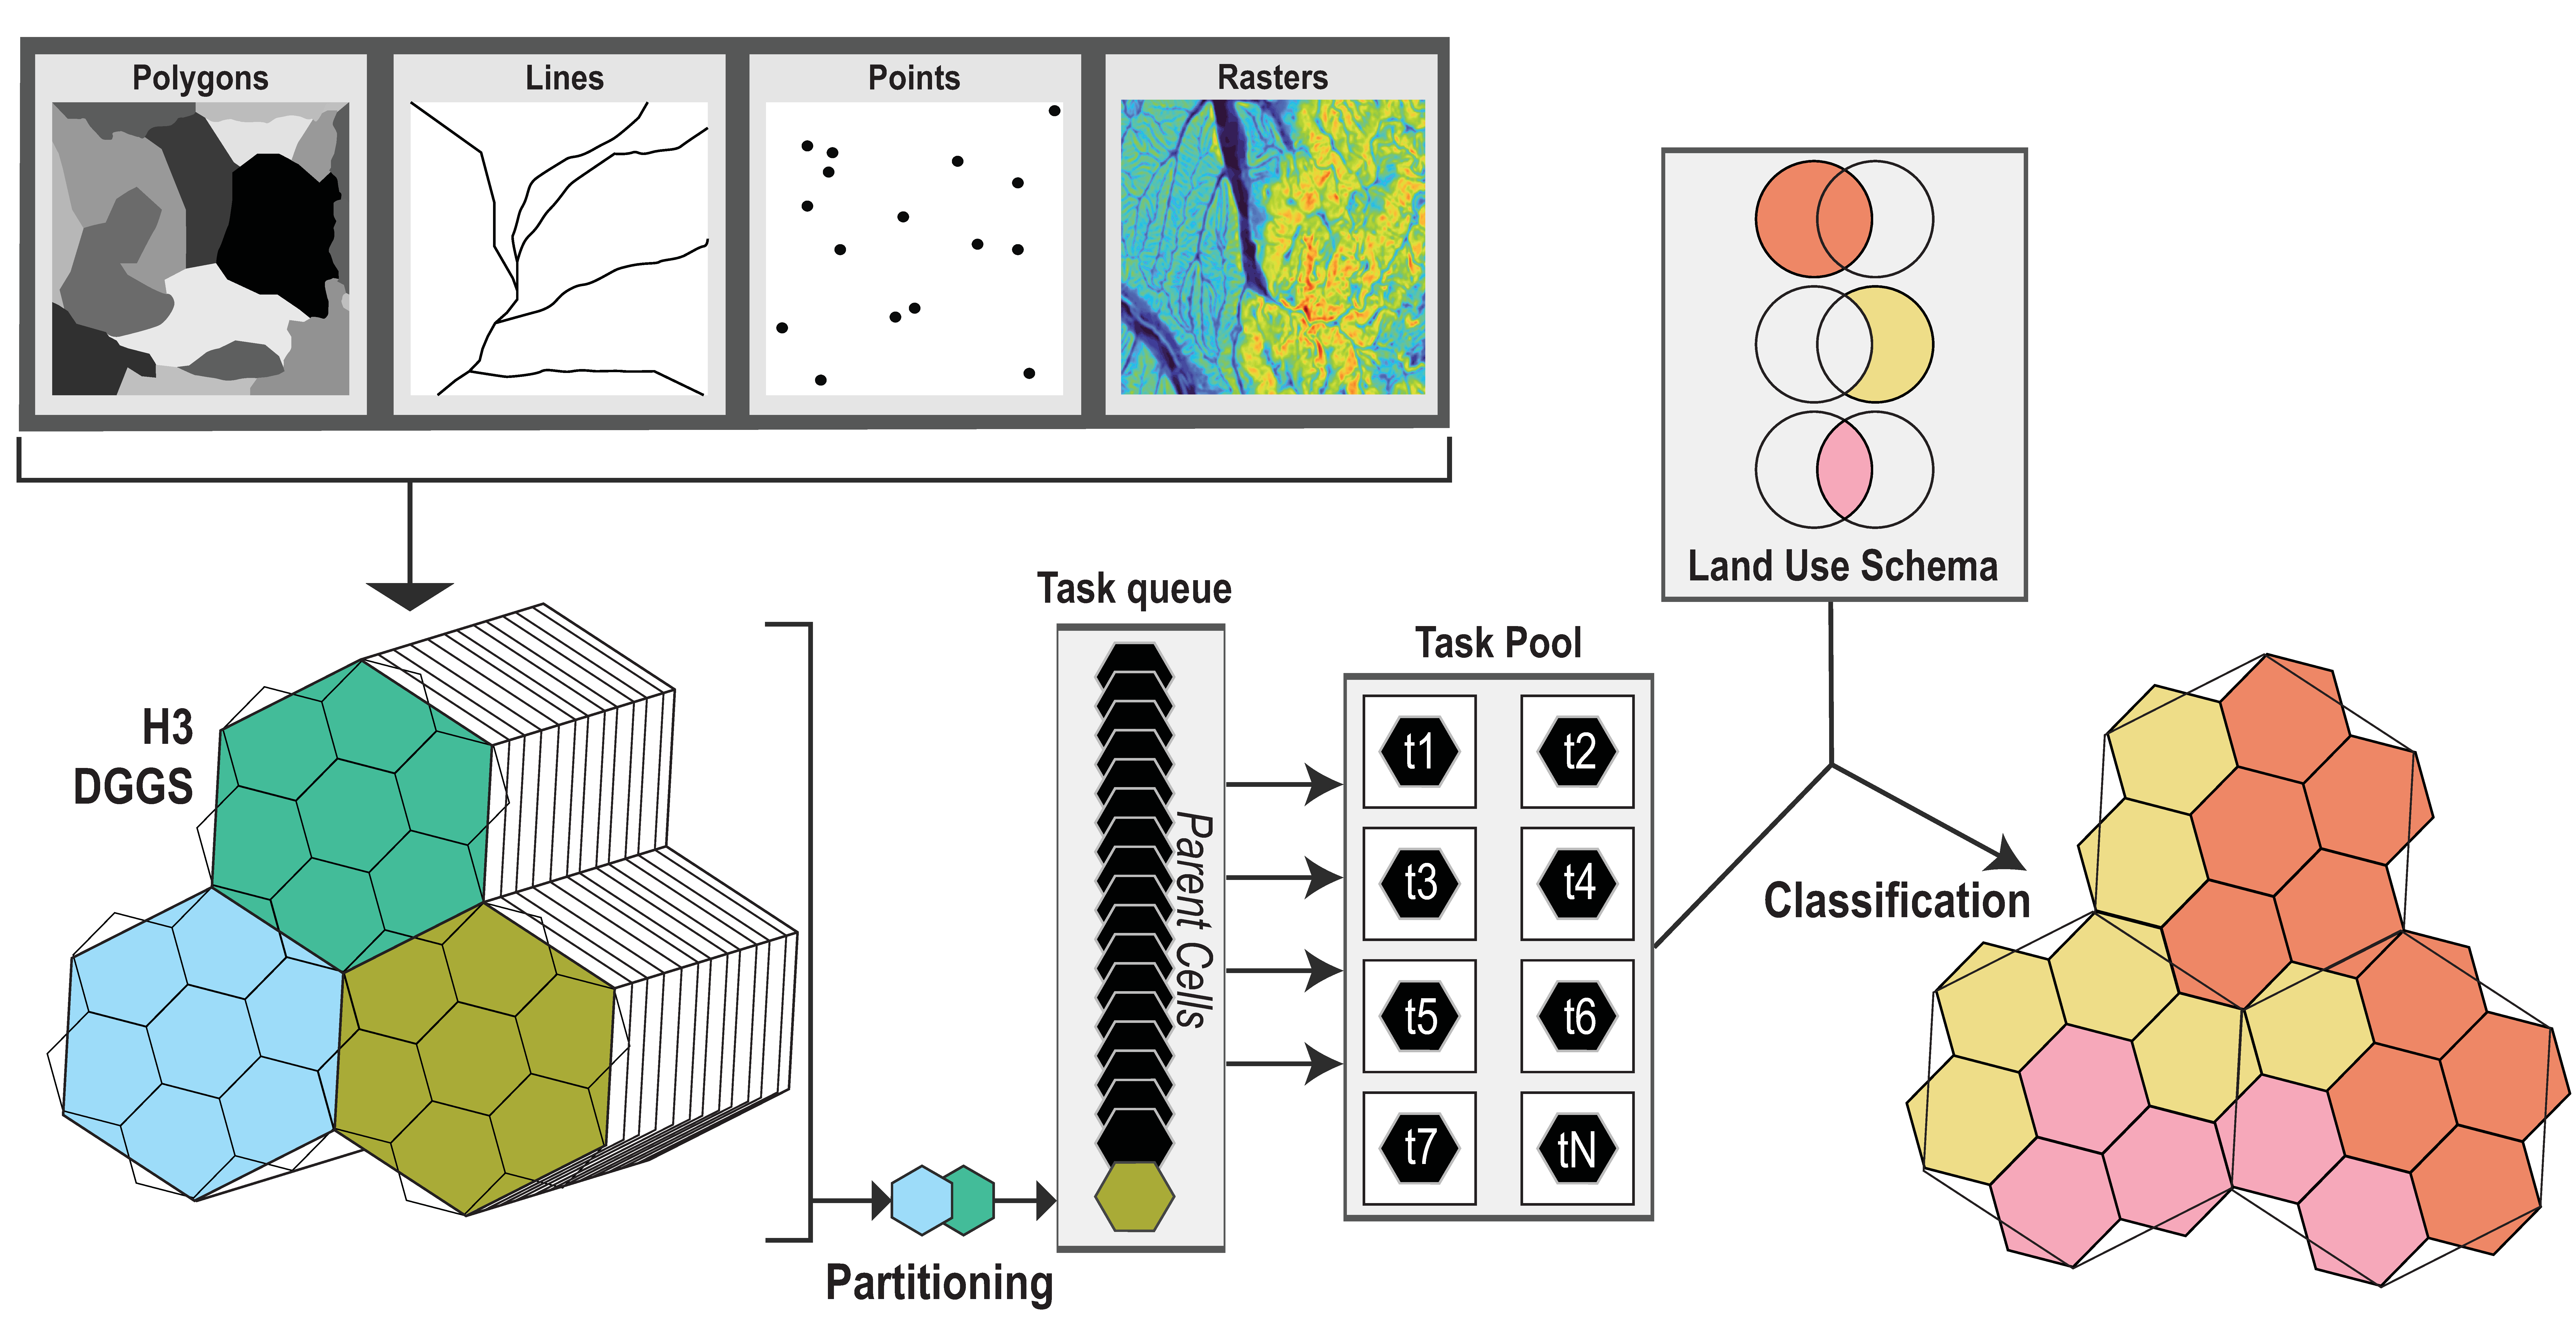
\includegraphics[width=0.6\linewidth]{images/GraphicalAbstract1.eps}
% \end{center}

\begin{keywords}
\Acl{DGGS}; \acl{GIS}; land-use mapping; horizontal scalability; data interoperability; reproducibility; benchmarking
\end{keywords}
%TC:endignore

\section{Introduction} % 2000 words

Digital land-use assignment, classification or mapping is the task of determining to which class a pixel or geographic feature belongs, among a set of predefined classes constituting a coherent system of land use classes.\footnote{For this paper, we put aside the related issue of determining an appropriate land-use assignment schemata or vocabulary of terms. Rather, we assume that an appropriate classification system exists and focus on how geospatial information can be effectively manipulated in order to produce data that adheres to such a schemata.} The decision is based on available data from a variety of sources, most commonly remotely sensed information (as in traditional land cover mapping) in conjunction with vector geospatial information \citep{rozenstein2011comparison}. \textit{Land-use} is (or should be) distinct from \textit{land cover} in that the land cover implies but does not necessarily entail a particular land-use \citep{fisher2005land,cihlar2001land}. For example, an area of improved grass pasture (land cover) may be used for different farm systems, multiple co-located uses, or even be abandoned (land-use).

Land-use maps are a key input for process models that describe physical properties of the world for analysis of pressures, changes and risk in the Earth's environmental systems \citep{bach2006accuracy,stehman1998design}. As records of dynamic landscape information, they are generated repeatedly and used as baselines for predictive models; they therefore must be reproducible. It is likewise important to have the ability to adjust the techniques of producing land-use information as new input data becomes available, or as new classification schema are required to answer novel questions. The technical efficiency of methods of producing geospatial land-use information is therefore an important question that is distinct from a choice of appropriate land-use schemata, or the accuracy of any derived information.

As it is demonstrably insufficient to rely \textit{only} on remotely-sensed geospatial data to classify land according to its use, geospatial data integration is a key problem in land-use mapping \citep{lillesand2015remote}. In the application of a land cover classification algorithm, the analyst is typically afforded coherent raster geospatial information across multiple spectral bands, and even across time (e.g. a datacube) \citep{kopp2019achieving}. However, the additional data necessary for land-\textit{use} mapping are likely to come from a wide variety of sources, including municipal authorities, conservation organisations, central government, independent research agencies, volunteered geospatial information, etc. \citep{rozenstein2011comparison}. There is no guarantee that these will be consistent in terms of coverage, format, data model, delivery protocol, spatial or temporal resolution, and how often they are updated.

Some of the significant problems that emerge when attempting to synthesise these data into land-use information are:

\begin{itemize}
    \item The fundamental incompatibility of the raster and vector geospatial data models \citep{piwowar1990integration,goodchild1994integrating}.
    \item Data artefacts that arise from precision error (e.g. at the boundary of infinite-precision objects) when performing geospatial union operations on vector geometries. \citep{schneider2003design,veregin1989error}
    \item The inefficiency of computation on infinite-precision vector geospatial objects (compared to a discrete grid) \citep{hojati2022giscience}.
\end{itemize}

We propose that the adoption of a \acf{DGGS} addresses these problems while affording additional benefits; but we do not attempt to argue that it is a panacea for all data integration issues. This paper will describe our approach using the hexagonal, hierarchical and geodesic Uber H3 \ac{DGGS} \citep{brodsky2018h3} as a means to integrating heterogeneous geospatial information. We will explain that the adoption of any \ac{DGGS} affords the opportunity for horizontal scaling for geospatial classification by using column-oriented data formats (e.g. Apache Parquet) which natively support the \ac{DGGS} data model \textit{without} an explicit understanding of the data structure as geospatial information. This can be done in such a way that the output can be presented in either the vector or raster data models and therefore does not require end users to adopt a \ac{DGGS} in order to use the output land-use data. As a stable reference grid, a \ac{DGGS} is an appropriate data structure for enhancing analytical reproducibility in \ac{GIS} \citep{purss2019datacubes,etherington2022}.

In this paper we also perform two benchmarking exercises to compare the performance of overlay and geographic object classification when using a \ac{DGGS} against the performance of equivalent vector- and raster-oriented workflows.

\section{Advantages of a \ac{DGGS} for land-use mapping} % 2000 words

A \ac{DGGS} is a system that uses a hierarchical tessellation of zones to partition and address the entire Earth. \citet{sahr2003geodesic} have shown how ``geodesic'' \acp{DGGS} (rather than quadtrees based on geographic coordinates) can be constructed, and thus meliorate distortion errors caused by map projection \citep{goodchild2018reimagining}.

The \ac{DGGS} data model is fundamentally different from the traditional vector \ac{GIS} data model, in the fact that geographic data is represented by collections of discrete zones\footnote{Terminology: `cells' are the unit of geometry in a \ac{DGGS}, and the geometry of the region of space-time occupied by a `zone' is a cell \citep{topic21}.} rather than geometries expressed by coordinates in a continuous space. Having a discrete geographic representation of space avoids the need for a computer to algorithmically determine the intersection of non-finite objects in a continuous space \citep{bentley1979algorithms,robertson2020integrated}. The discretisation of space ultimately allows for predictable and faster computes on congruent, aligned data \citep{dutton1989modelling}.

\subsection{Scalability}

\begin{figure}[t]
    \centering
    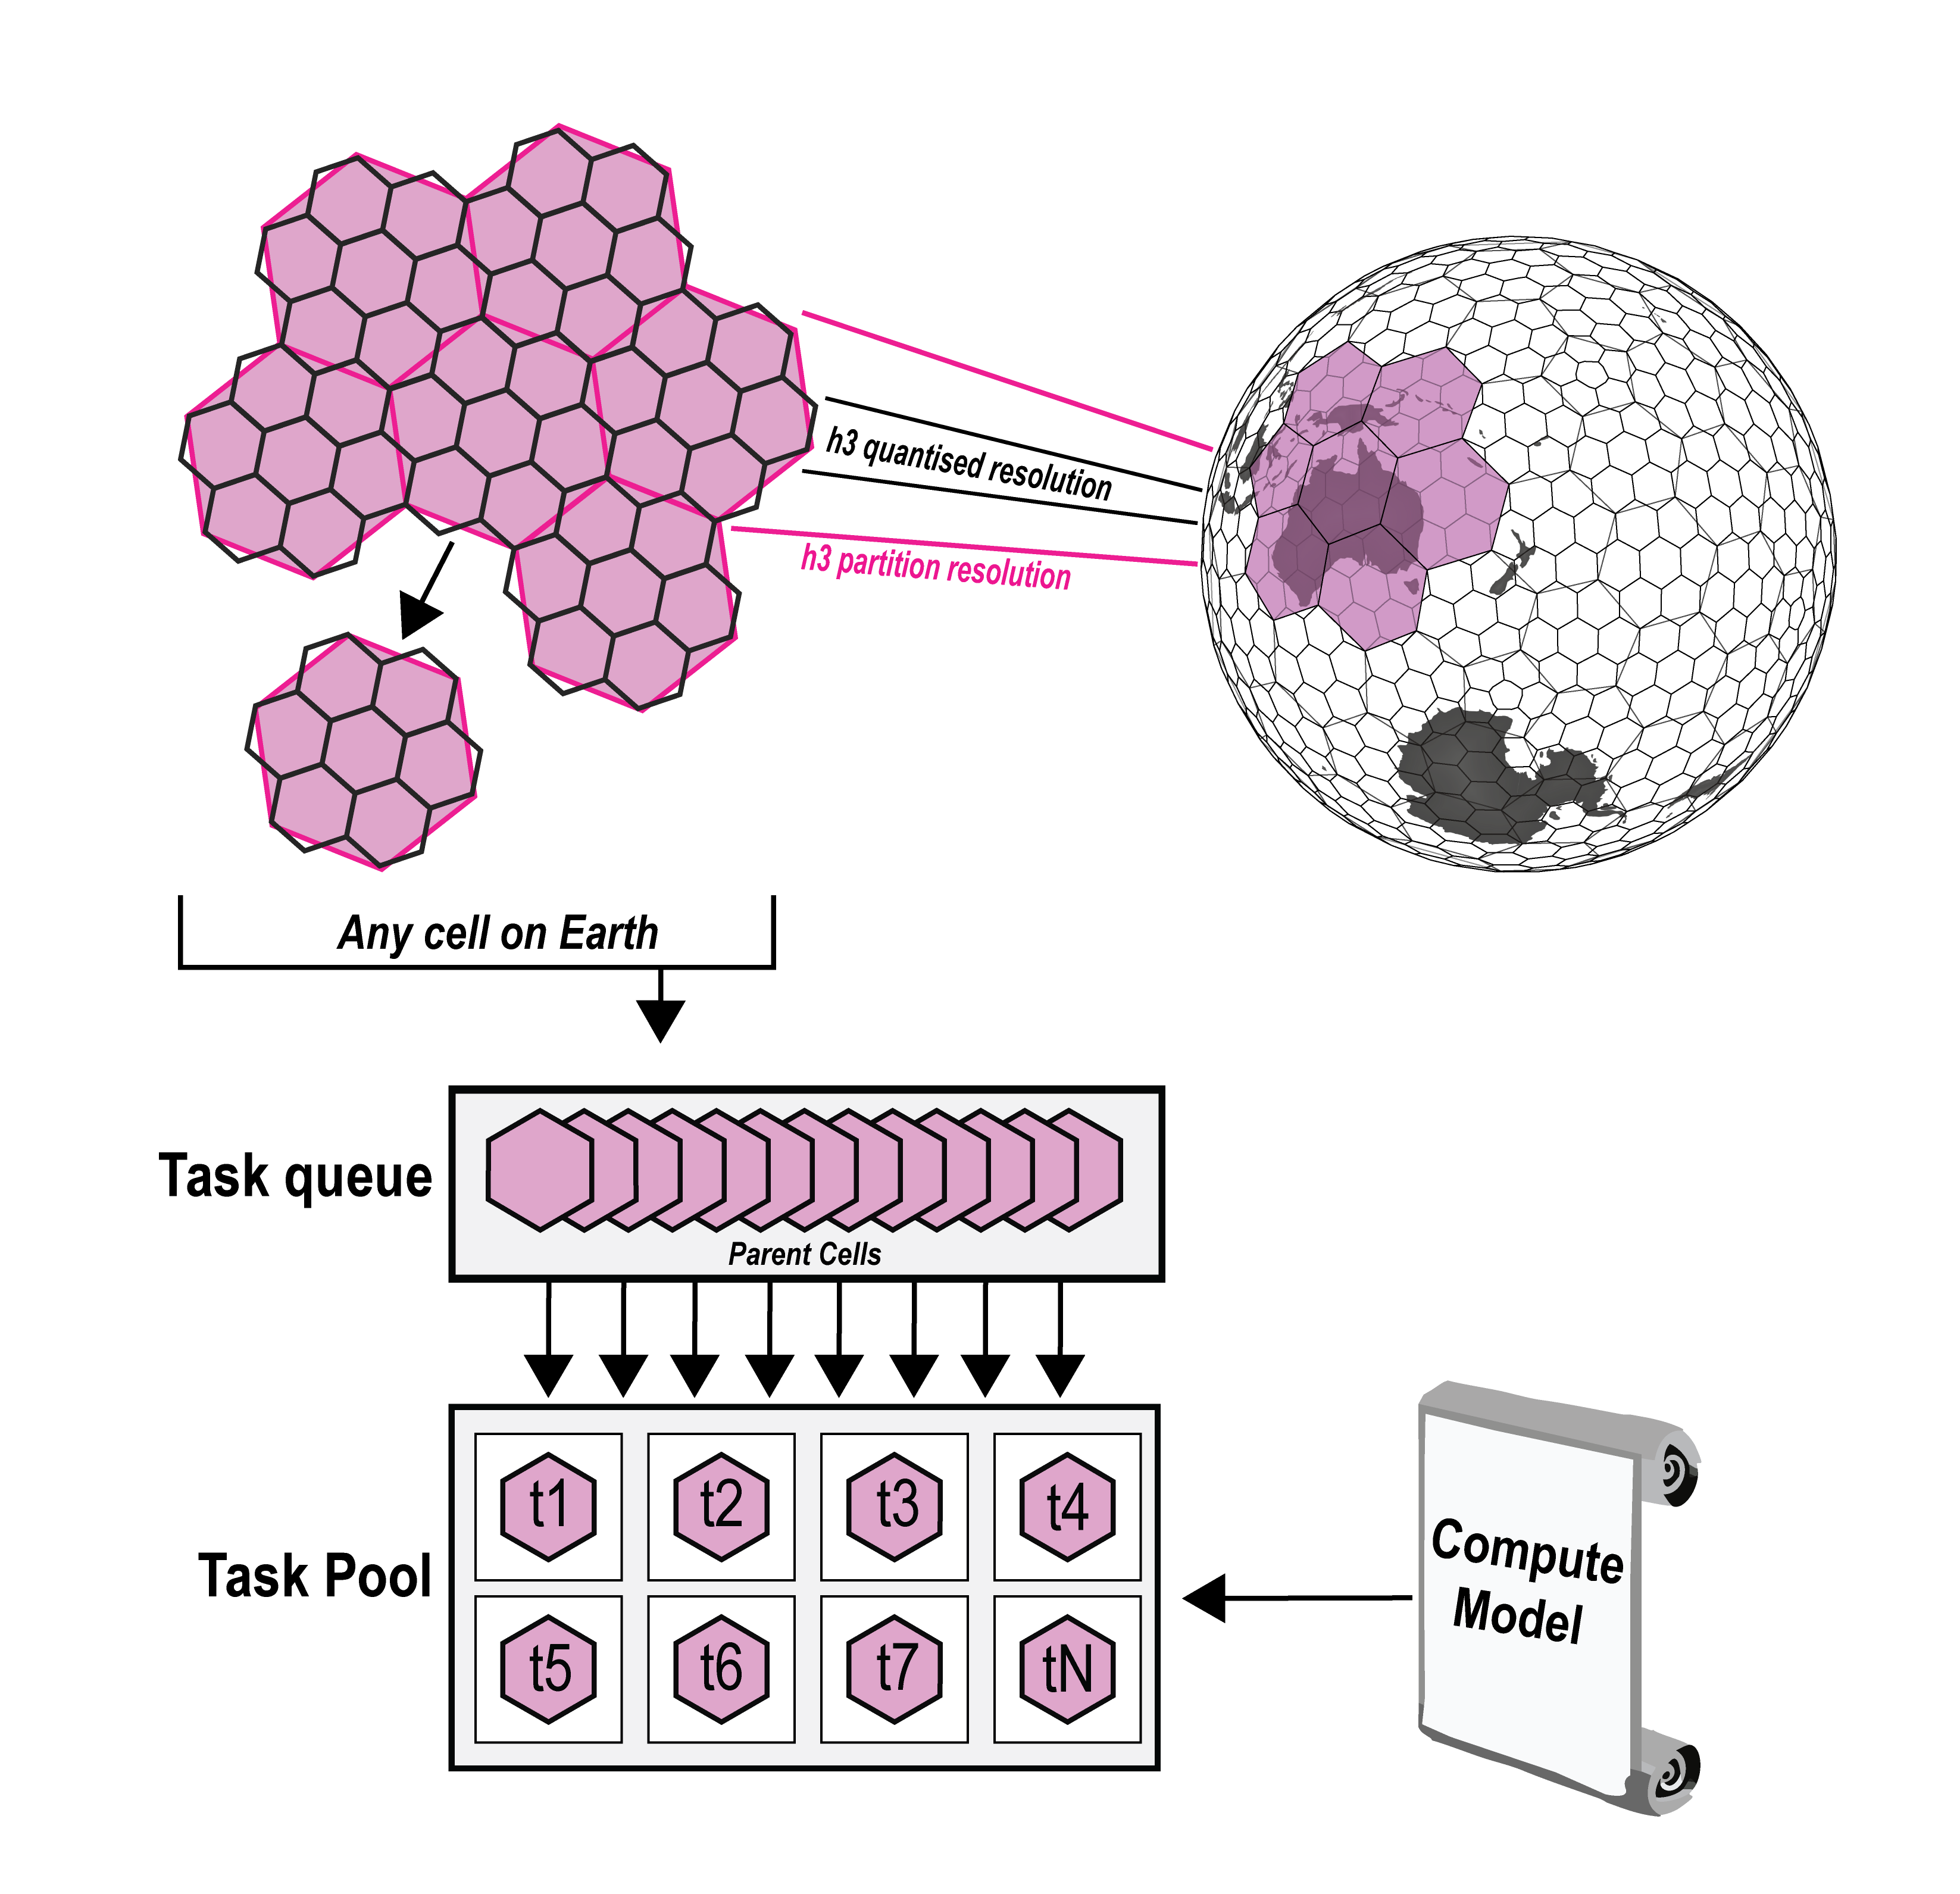
\includegraphics[width=0.65\linewidth]{images/DGGS_lu-02.eps}
    \caption{The \ac{DGGS} data model is suitable for horizontal scaling. Spatial partitioning is inherent in the structure of a \ac{DGGS}. Zones at a particular resolution (black outlines) can be partitioned by a common ancestor (pink outlines) at an appropriate offset (here, just one level). Combinational logic (map classification) can then be applied in parallel across all available compute cores to evenly-partitioned data.}
    \label{fig:Scalable}
\end{figure}

The \ac{DGGS} data model is hierarchical. Each zone is subject to a recursive pattern whereby child zones are of progressively finer resolution. This can be expressed as a series of space-partitioning parent-child zone relationships. It is possible to then immediately partition data across multiple nodes for scalability (Figure \ref{fig:Scalable}). As this can be determined instantaneously by using a ``parent'' offset to spatially partition data, this is more efficient than constructing (and re-constructing) a quadtree index. (This is not possible with the subset of \acp{DGGS} that do not have a nested cell refinement strategy, which we do not consider in this paper.)

The partitions are then added to a task queue, for processing in a task pool that scales with the number of cores available, perhaps in a distributed system. This assumes that each partition can be treated independently. If this is not the case---perhaps if the \textit{neighbourhood} of a zone is relevant to the classification---then the partitioning pattern may still be used, but the central partition will need to be passed to the compute node alongside its neighbouring partitions up to some relevant distance from itself. \acp{DGGS} allow for the efficient enumeration of zone neighbours to facilitate this access pattern.

A parent offset of six would achieve partition sizes of $a^{6}$ where $a$ is the aperture of the \ac{DGGS}, or how many child zones there are to each parent zone; this is 7 in the case of H3, making each partition 117\,649 zones. This fixed partition size has the advantage of ensuring balanced and predictable memory allocation for each partition. Partition keys are the parent zone IDs, and we have found this pattern effective with both partitioned tables in PostgreSQL (using list partitioning) and also as a partition key for storing data in Parquet files (or other column-oriented data structures).

Partition keys are usually used to limit the results of particular queries by exploiting knowledge of common access patterns \citep{abadi2008column}. For example, partitioning data into daily partitions, such that queries for particular days in the year will only need to read and process data for one partition. However in the case of land-use mapping it is still usually necessary to process the entire set of data (although regional or local maps built from national data will benefit). The benefit then is to exploit the partitioned data structure to process the entire dataset in parallel, progressively while still scaling with available compute nodes.

\subsection{Data interoperability}

\begin{figure}[t]
    \centering
    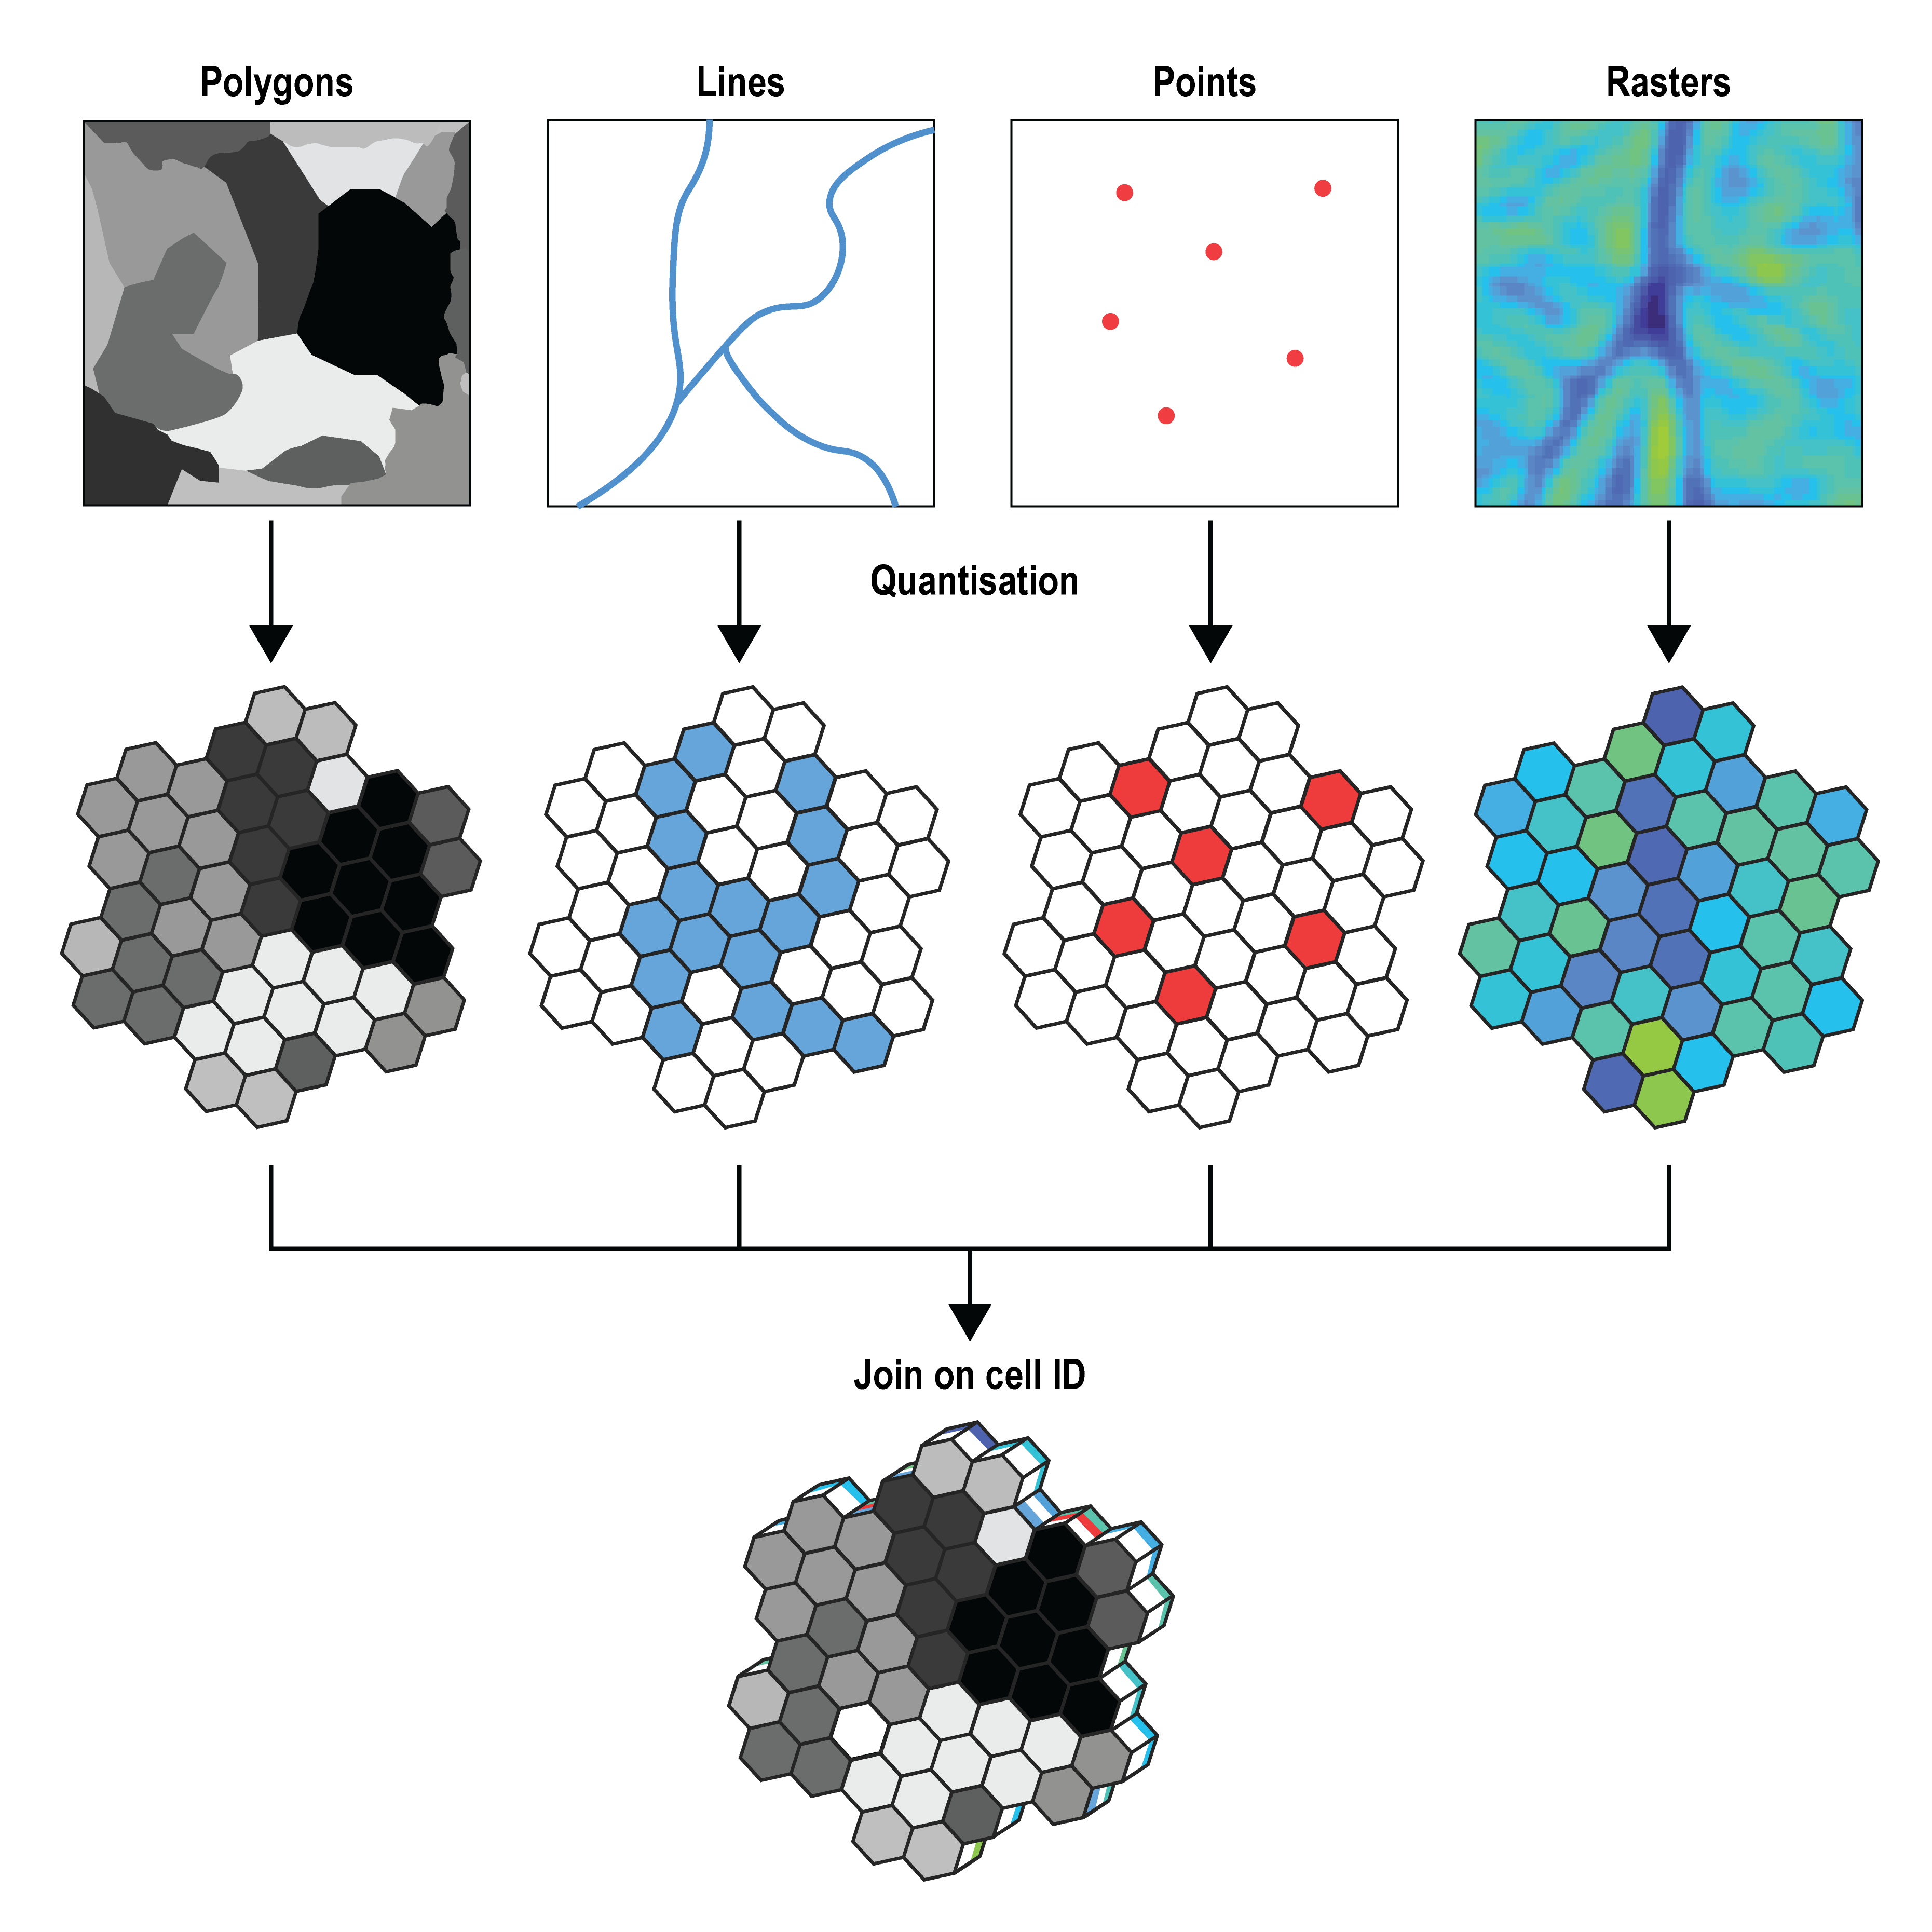
\includegraphics[width=0.65\linewidth]{images/DGGS_lu-01.png}
    \caption{Data quantisation with a \ac{DGGS}. Both vector and raster data may be transformed. Quantised data from disparate inputs can be related using the \ac{DGGS} zone ID in an implicit spatial join.}
    \label{fig:Interoperable}
\end{figure}

Land-use mapping tasks can benefit from geospatial information available in both the raster and vector data models. Traditionally, to work across these data models it is necessary to decide on a workflow that adopts either the raster or vector data models, and convert all data to the same model \citep{winter1998bridging,wade2003comparison}. That is: raster data may be vectorised, or vector data may be rasterised. There are various decisions that need to be made when performing such conversions. For example, continuous raster data can be converted to vector data by computing appropriate `zonal statistics' \citep{zhang2015efficient,singla2018distributed}, among other techniques for discrete raster data. Vector data can be rasterised more directly, and indeed in a manner that is conceptually equivalent to how vector data is indexed to a \ac{DGGS}.

When indexed to a \ac{DGGS}, geospatial data originally available as raster or vector data becomes associable, using a zone ID as a join key \citep{dutton1989modelling,sahr2019central}. Some loss of fidelity is possible according to the chosen \ac{DGGS} zone resolution. However some information can be retained that is typically difficult to retain when using a raster-based workflow: the shape and attributes of overlapping vector features; sequential information (the direction of linear features); self-intersection (a line that loops on itself could be represented by an ordered sequence of zones that may repeat).   

\subsection{Reproducibility}

\begin{figure}[t]
    \centering
    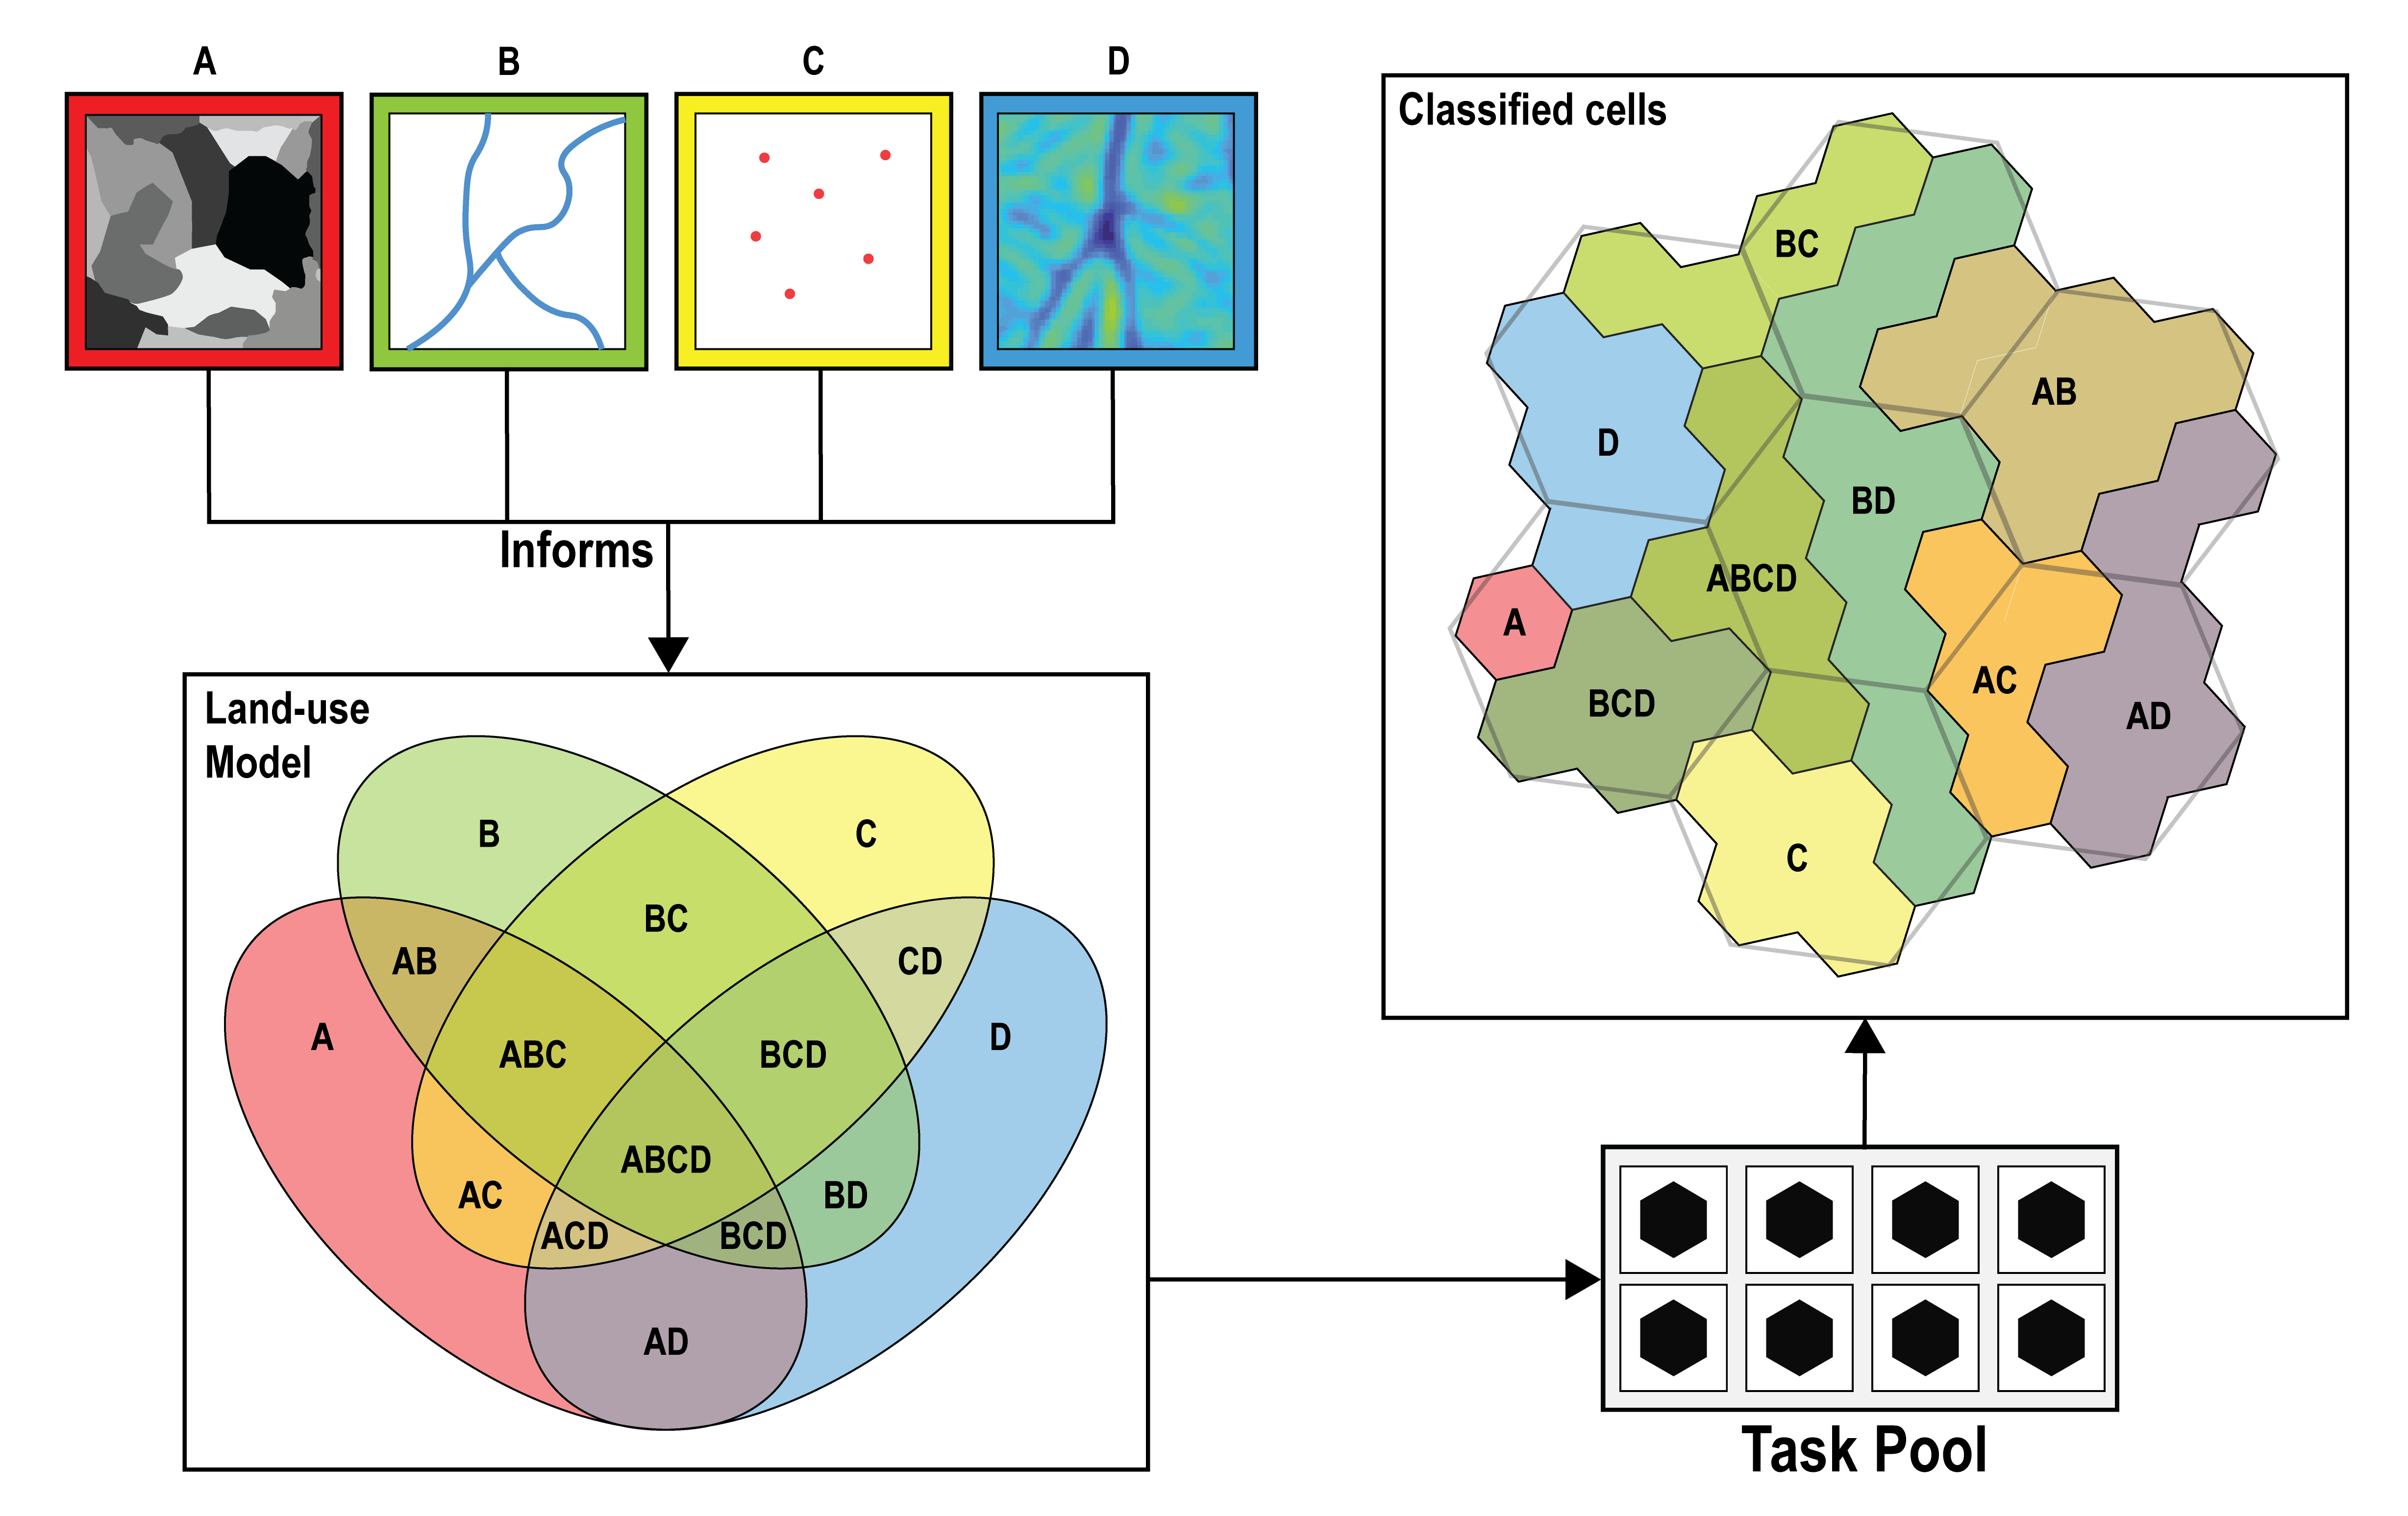
\includegraphics[width=0.65\linewidth]{images/DGGS_lu-03.png}
    \caption{Land classification tasks can be represented as Venn (or Euler) diagrams, in which particular spatial relationships between geospatial features are meaningful and can be labelled. Most commonly, intersection (or non-intersection) is meaningful, but adjacency may also be relevant. Attribute joins using \ac{DGGS} zone IDs are equivalent to spatial intersection. This is efficient to compute, which allows the mapping rules to be (re-)developed iteratively and even interactively.}
    \label{fig:Reproducible}
\end{figure}

Land-use mapping is often performed by combining available geospatial data with sets of rules that represent relationships between these data with various attributes (Figure \ref{fig:Reproducible}). An example might be that a ``commercial dairy farm'' is any a) parcel of land with freehold or leasehold title that is b) largely covered with improved pasture, c) has a consent for discharging dairy effluent, and d) has a cattle stocking rate above some threshold. Other information may add confidence, such as the presence or absence of a milking shed. At a finer scale, sub-areas of the farm may be further sub-classed, recognising the co-location of waterways, remnant native forest, farm infrastructure, and residences. Classification systems may be developed top-down (class design considered first) or bottom-up (available data considered first), but ultimately geospatial data must be combined in order to produce a derived dataset: a land-use map \citep{rutledge2009geospatial}.

This process of determining how components of land-use information may be a manual, iterative process; or it could be approached as a supervised or deep learning problem. As more data is added to the process, and refinements are made to attribute queries to more specifically select land that meets relevant criteria, the set of rules becomes complex. Even redundant information (i.e. information from independent sources about the same thing) may be combined to build confidence in the identification of a particular geographic area as belonging to a particular land-use class.

During development, an analyst will combine layers, then examine whether the classified output appears sensible, and then iterate this process for more input layers to achieve greater accuracy, greater precision, or to realise more land-use classes. Only after performing this iterative task for many or all available inputs will an analyst attempt a complete, rigorous verification of the derived land-use information. 

This iterative process is an attempt at extracting meaningful and succinct information from multivariate data. It is challenging because the total number of possible combinations of the data grows exponentially with the dimensionality of the set of input data (the number of datasets, and the number of distinct feature attribute values within each dataset) \citep{behrisch2014feedback}. The automated reproduction of any derived land-use map is critical to achieving confidence in the data, and so it can be verified by independent analysts \citep{etherington2022,baker2016}.

The ability to reproduce a dataset is therefore important both \textit{during} and \textit{after} a land-use data artefact has been made. During, because an analyst benefits from a rapid feedback loop; and after because verification depends on the feasible and precise re-production of the data from source.

During production, an analyst can more efficiently work with a short feedback loop between creating or changing a map classification rule, and seeing the outcome of that change. A \ac{DGGS} allows an analyst to accomplish this by adapting the resolution of the analysis, perhaps using a low resolution for rapid iteration. An analyst can also limit the scope of the computation by limiting the reproduction to a particular (spatial) partition, perhaps a problematic or representative area, and avoid continual recomputation over large areas at high resolutions.

After production, the general efficiency of the classification process makes the output easier to reproduce by independent analysts (provided the source data, and the map classification rules are published with a permissive license), or simply to update the data to begin a temporal series of land-use change.

\section{Application} % 1000 words

% TODO - should this be rephrased to make it not sound self-referential? How does this affect blind peer review?
\subsection{Demonstration land-use map}

We applied these ideas when developing a land-use map for Northland, a region of New Zealand of \qty{12500}{\km\squared} and 200\,000 people \citep[see][]{law2023}. We implemented version 8 of the \ac{ALUM} classification system, which has a Creative Commons license. The \ac{ALUM} classification goes beyond the specification of a hierarchical schemata of land-use classes, and includes guidelines for the mapping of land use from aerial imagery and ancillary information, and a vocabulary of commodities and management practices used to add detail beyond the available classes. The use of a \ac{DGGS} is not part of the \ac{ALUM} specification.

The production of this layer involved the integration of 48 different geospatial layers from many sources. Both raster and vector data types were included. The \ac{ALUM} classification system has over 200 classes at the tertiary level of the hierarchy; most but not all of these were realised for Northland. (Many of the unrealised classes were specifically Australian and were not applicable in New Zealand.)

The procedure for creating this land-use map involved an intermediate mapping of each \ac{DGGS} zone as each of the output classes, with varying degrees of confidence. The final classified map was then determined through a deterministic prioritisation process that combines: the qualitative confidence score (which captures trust in particular data sets and corroboration among multiple data sets); data currency; and geographic scale.

The adoption of the \ac{DGGS} ensured rapid prototyping through efficient combinational analysis and data partitioning, i.e. by being able to combine the input datasets and to apply expensive classification logic in parallel. The fixed precision of the \ac{DGGS} for some layers resulted in lower (but acceptable) fidelity and yet avoided the creation of innumerable sliver polygons that would have been derived from overlaying the large number of data sets with arbitrary coordinate precision. The system enabled us to dynamically aggregate the output to any particular spatial unit (e.g. property parcel, or watershed)---by performing an aggregation on an appropriate input feature ID---or none (i.e. individual \ac{DGGS} zones).

Apart from specifying inputs, detailing any input data transformations, and writing map classification rules with a declarative language (\ac{SQL}), the process was automated. Automation provided rapid prototyping, perfect reproducibility, and the ability to integrate updates to source datasets over the lifetime of the project.

Ultimately two data artefacts were created: property parcels encoded with the dominant land-use across the parcel (Figure~\ref{fig:NRC-ALUM}; determined by a \texttt{GROUP BY} statement over \ac{DGGS} zones with the same parcel ID), and a \ac{DGGS} zone-level dataset with each zone's land-use and ancillary data (such as various climate variables, elevation, and slope). The latter allowed for other data to be added as required (i.e. the attribute table can be widened) by indexing more data to the same DGGS.

\begin{figure}[t]
    \centering
    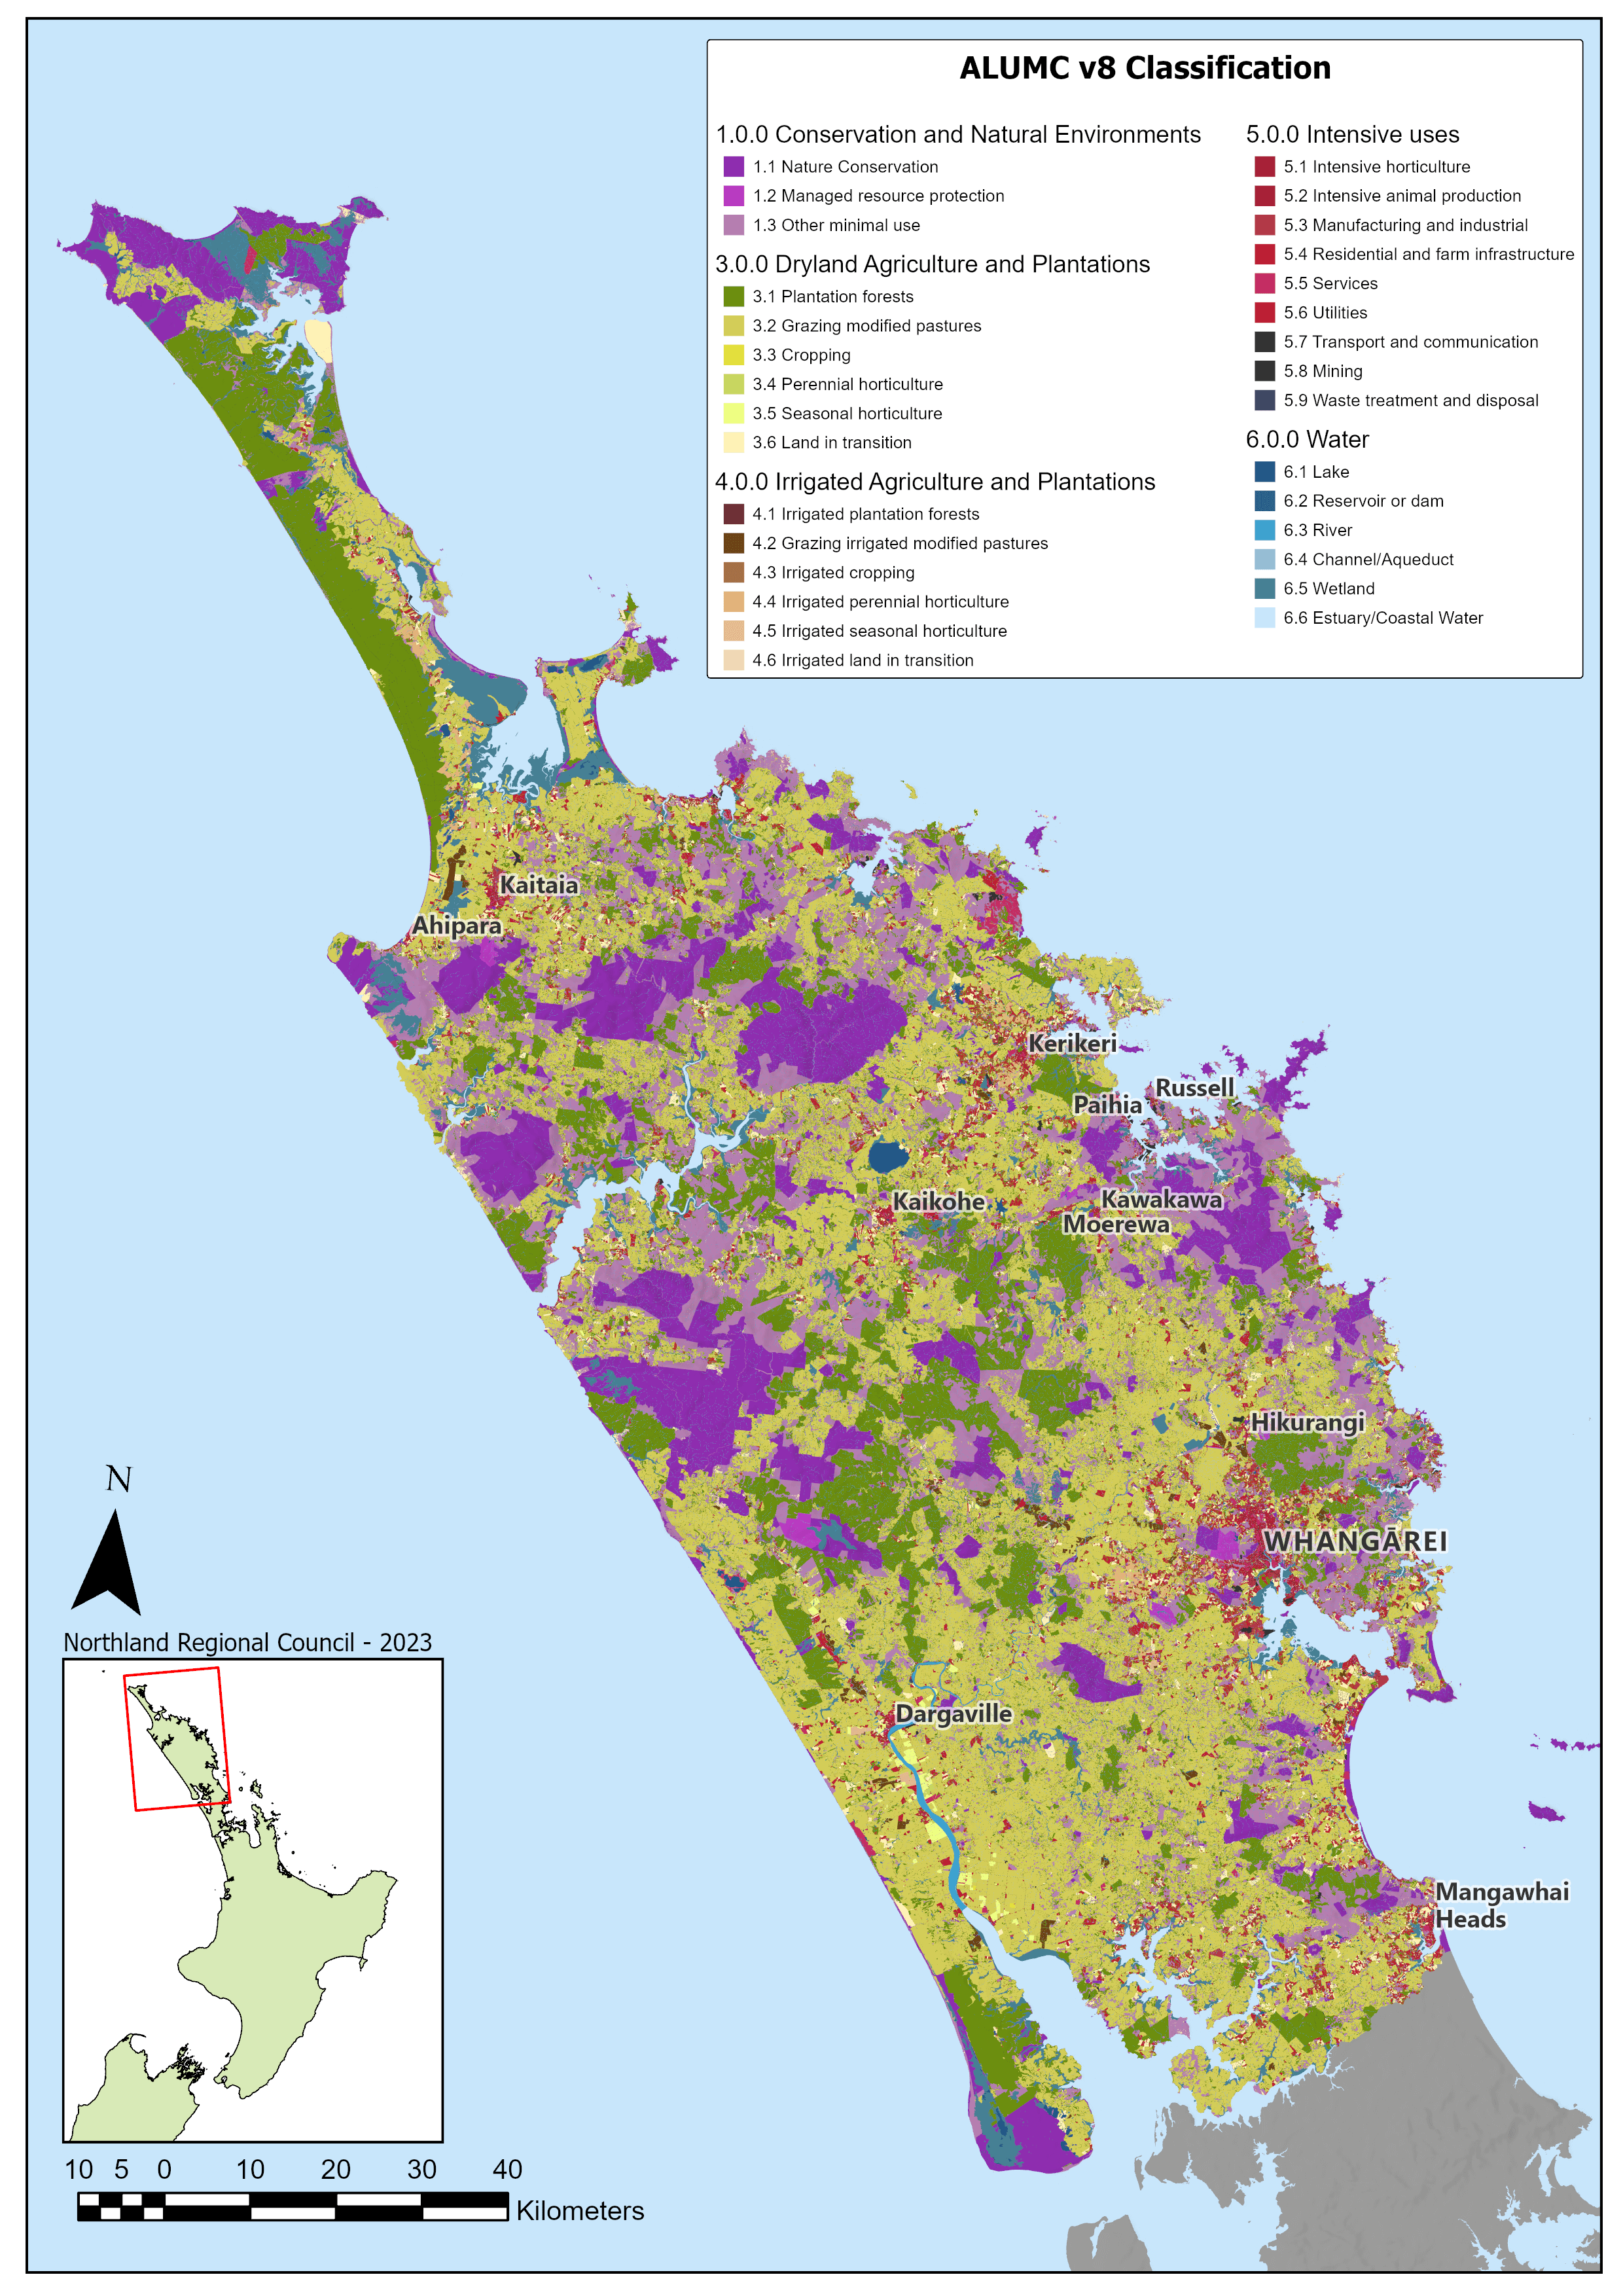
\includegraphics[width=1\linewidth]{images/NRC_ALUM.png}
    \caption{Land-use map of Northland, New Zealand using the H3 \ac{DGGS}. The map classification was performed to the tertiary level of the \ac{ALUM} classification hierarchy where data supported it, but only the secondary level is shown here for ease of comprehension. Reproduced from \citet{law2023}.}
    \label{fig:NRC-ALUM}
\end{figure}

\subsection{Performance benchmarking}

We designed a benchmarking experiment to compare a land-use mapping workflow using either vector data, or data indexed to a \ac{DGGS}. We then designed a similar experiment using raster data as input. Evaluating the performance of \ac{DGGS} for common \ac{GIS} tasks is one of the four \ac{GISc} research challenges for \acp{DGGS} recently identified by \citet{hojati2022giscience}. Few \ac{DGGS} benchmarking examples exist in the literature. Ensuring these comparisons are fair is somewhat fraught, due to the fundamental difference in object representation between the DGGS, vector, and raster data models; and because any operations on the traditional data models will benefit from many existing optimisations \citep{hojati2022giscience}. In the case of land-use mapping, we can design data-model-specific workflows to produce comparable outputs from identical (random) inputs, and measure the computational time.

\subsubsection{Vector}

We generated 500 random vector coverages, using a random distribution of points over a fixed extent, and calculated Voronoi polygons for each case. Each polygon in each coverage was randomly assigned a 0 or 1 value and then dissolved accordingly. These data were then spatially joined (union), and a (nonsense) map classification logic was applied to the unioned output. This classification required the Boolean value of all overlapping features to be summed, then that value was used as input for a series of functions that return a Boolean value. These functions are meaningless for land-use mapping, but are instructive in this case because they require at least some form of computation to mimic a meaningful map classification. These functions determine whether that sum is: a prime number; a perfect number; a triangular, square, pentagonal, or hexagonal number; or a Fibonacci number. Each unique combination of the eight resultant Boolean values was then considered a distinct "class" akin to a distinct land-use type.

To compare this to a \ac{DGGS} workflow, we first needed to perform the additional conversion step of indexing each input vector Voronoi polygon geometry to a fixed zone resolution. A polygon filling algorithm is implemented through the H3 Python bindings, which we used through H3-Pandas, where it is termed `polyfilling'.\footnote{\url{https://h3-pandas.readthedocs.io}} We then performed an attribute join on \ac{DGGS} zone ID, which is implicitly a spatial join but requires no explicit consideration of geometric intersection. The same map classification logic was then applied as in the vector baseline. Some further optimisations that could have been applied were not (such as caching the classification function outputs for the set of integer inputs) in order to avoid complicating the comparison.

\begin{figure}[t]
    \centering
    % \resizebox{25pc}{!}{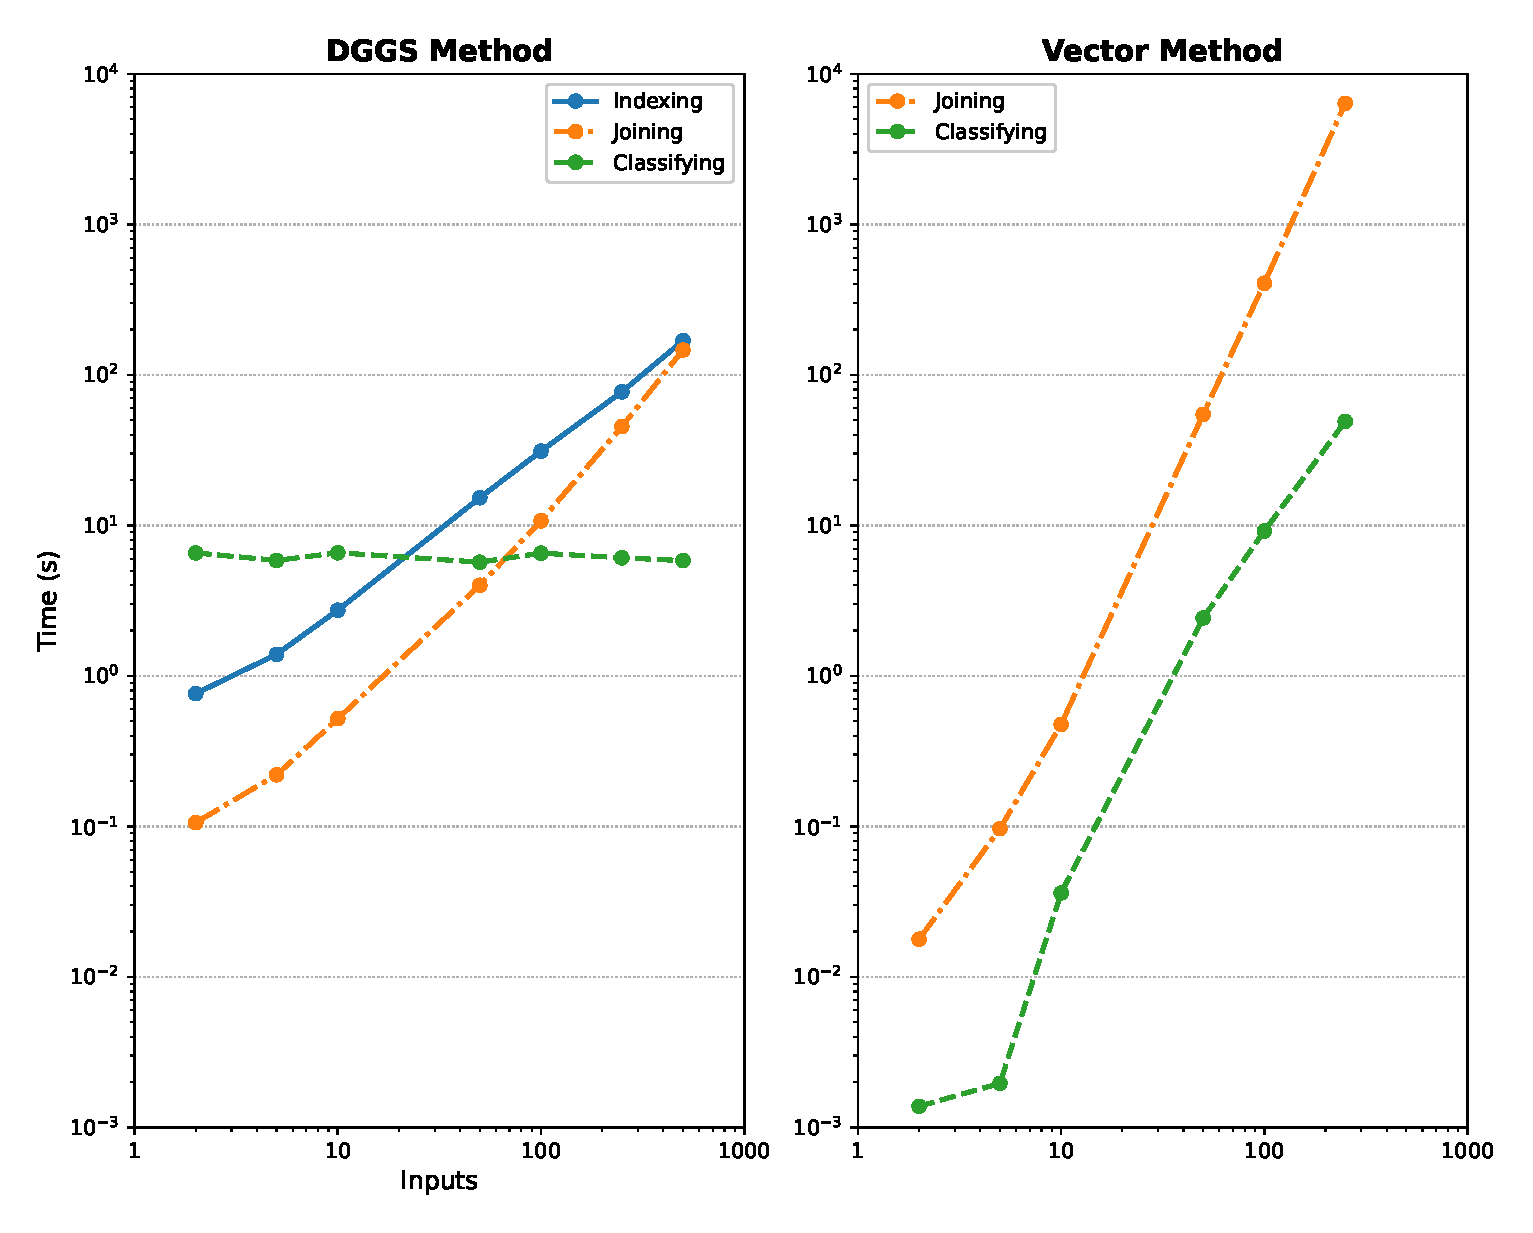
\includegraphics{images/vector-results.eps}}
    % 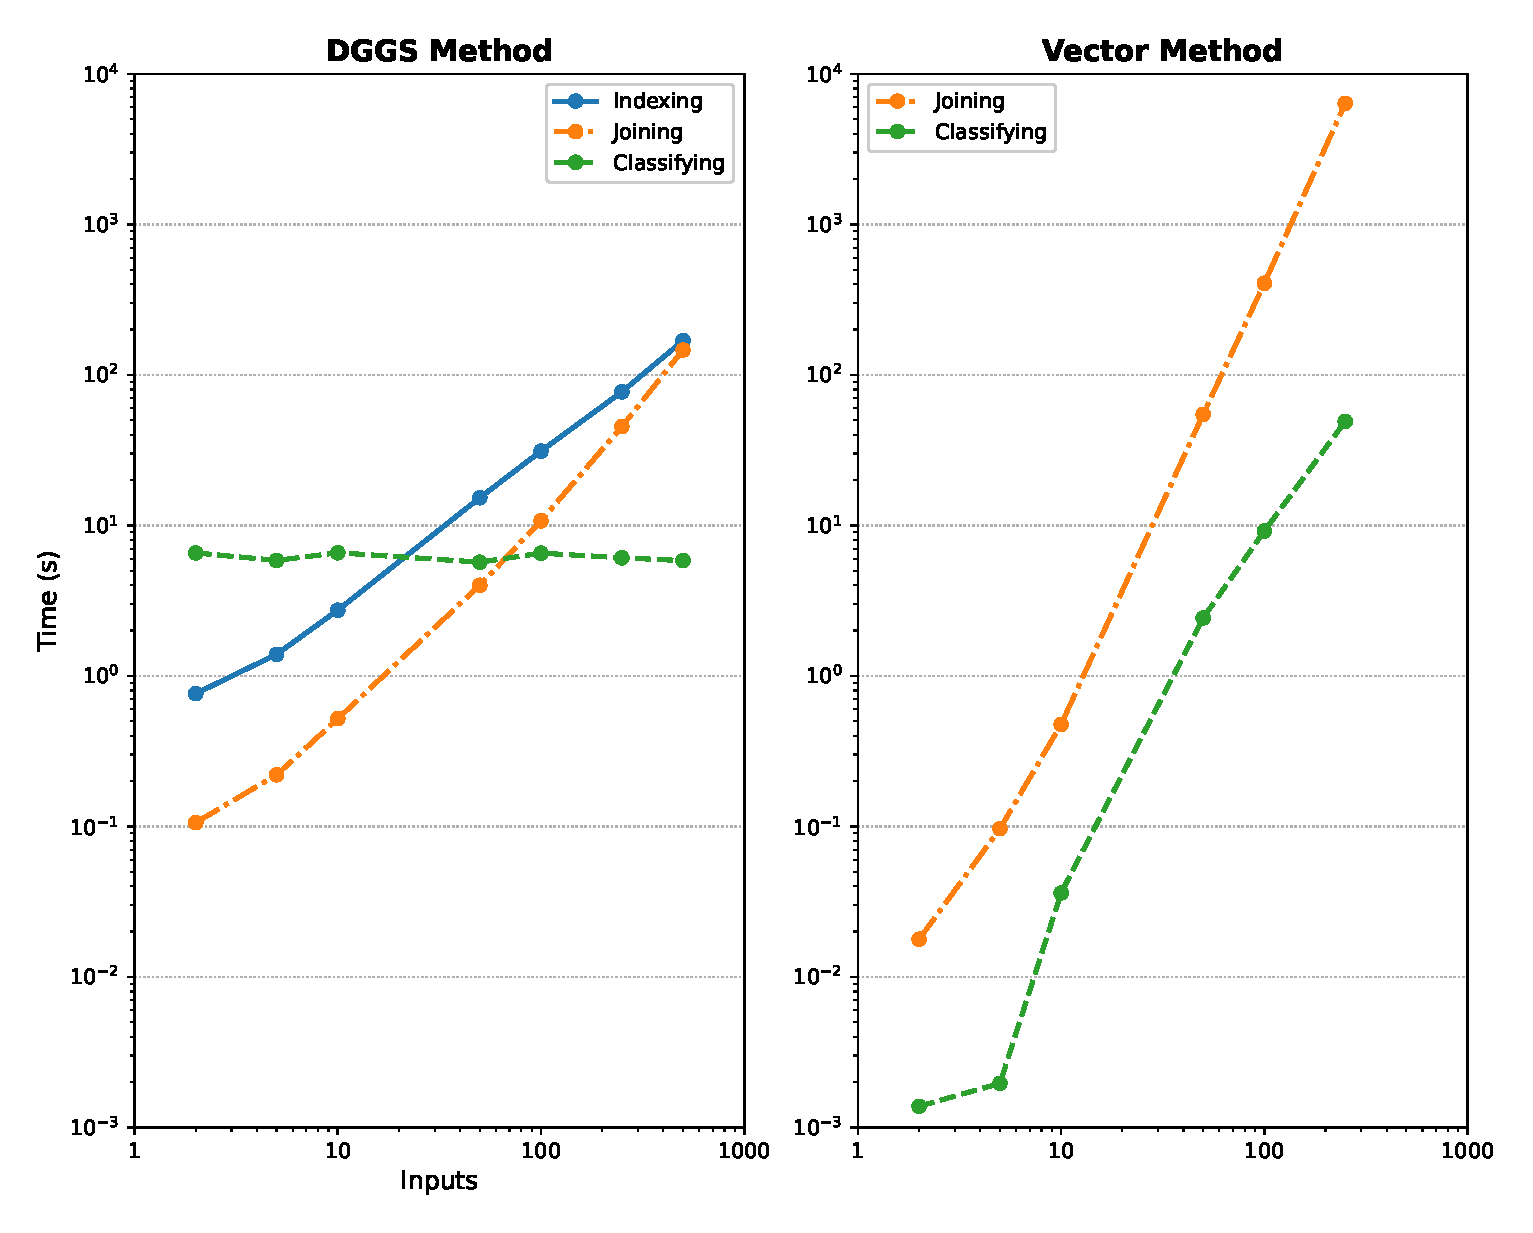
\includegraphics[width=0.85\linewidth]{images/vector-results.eps}
    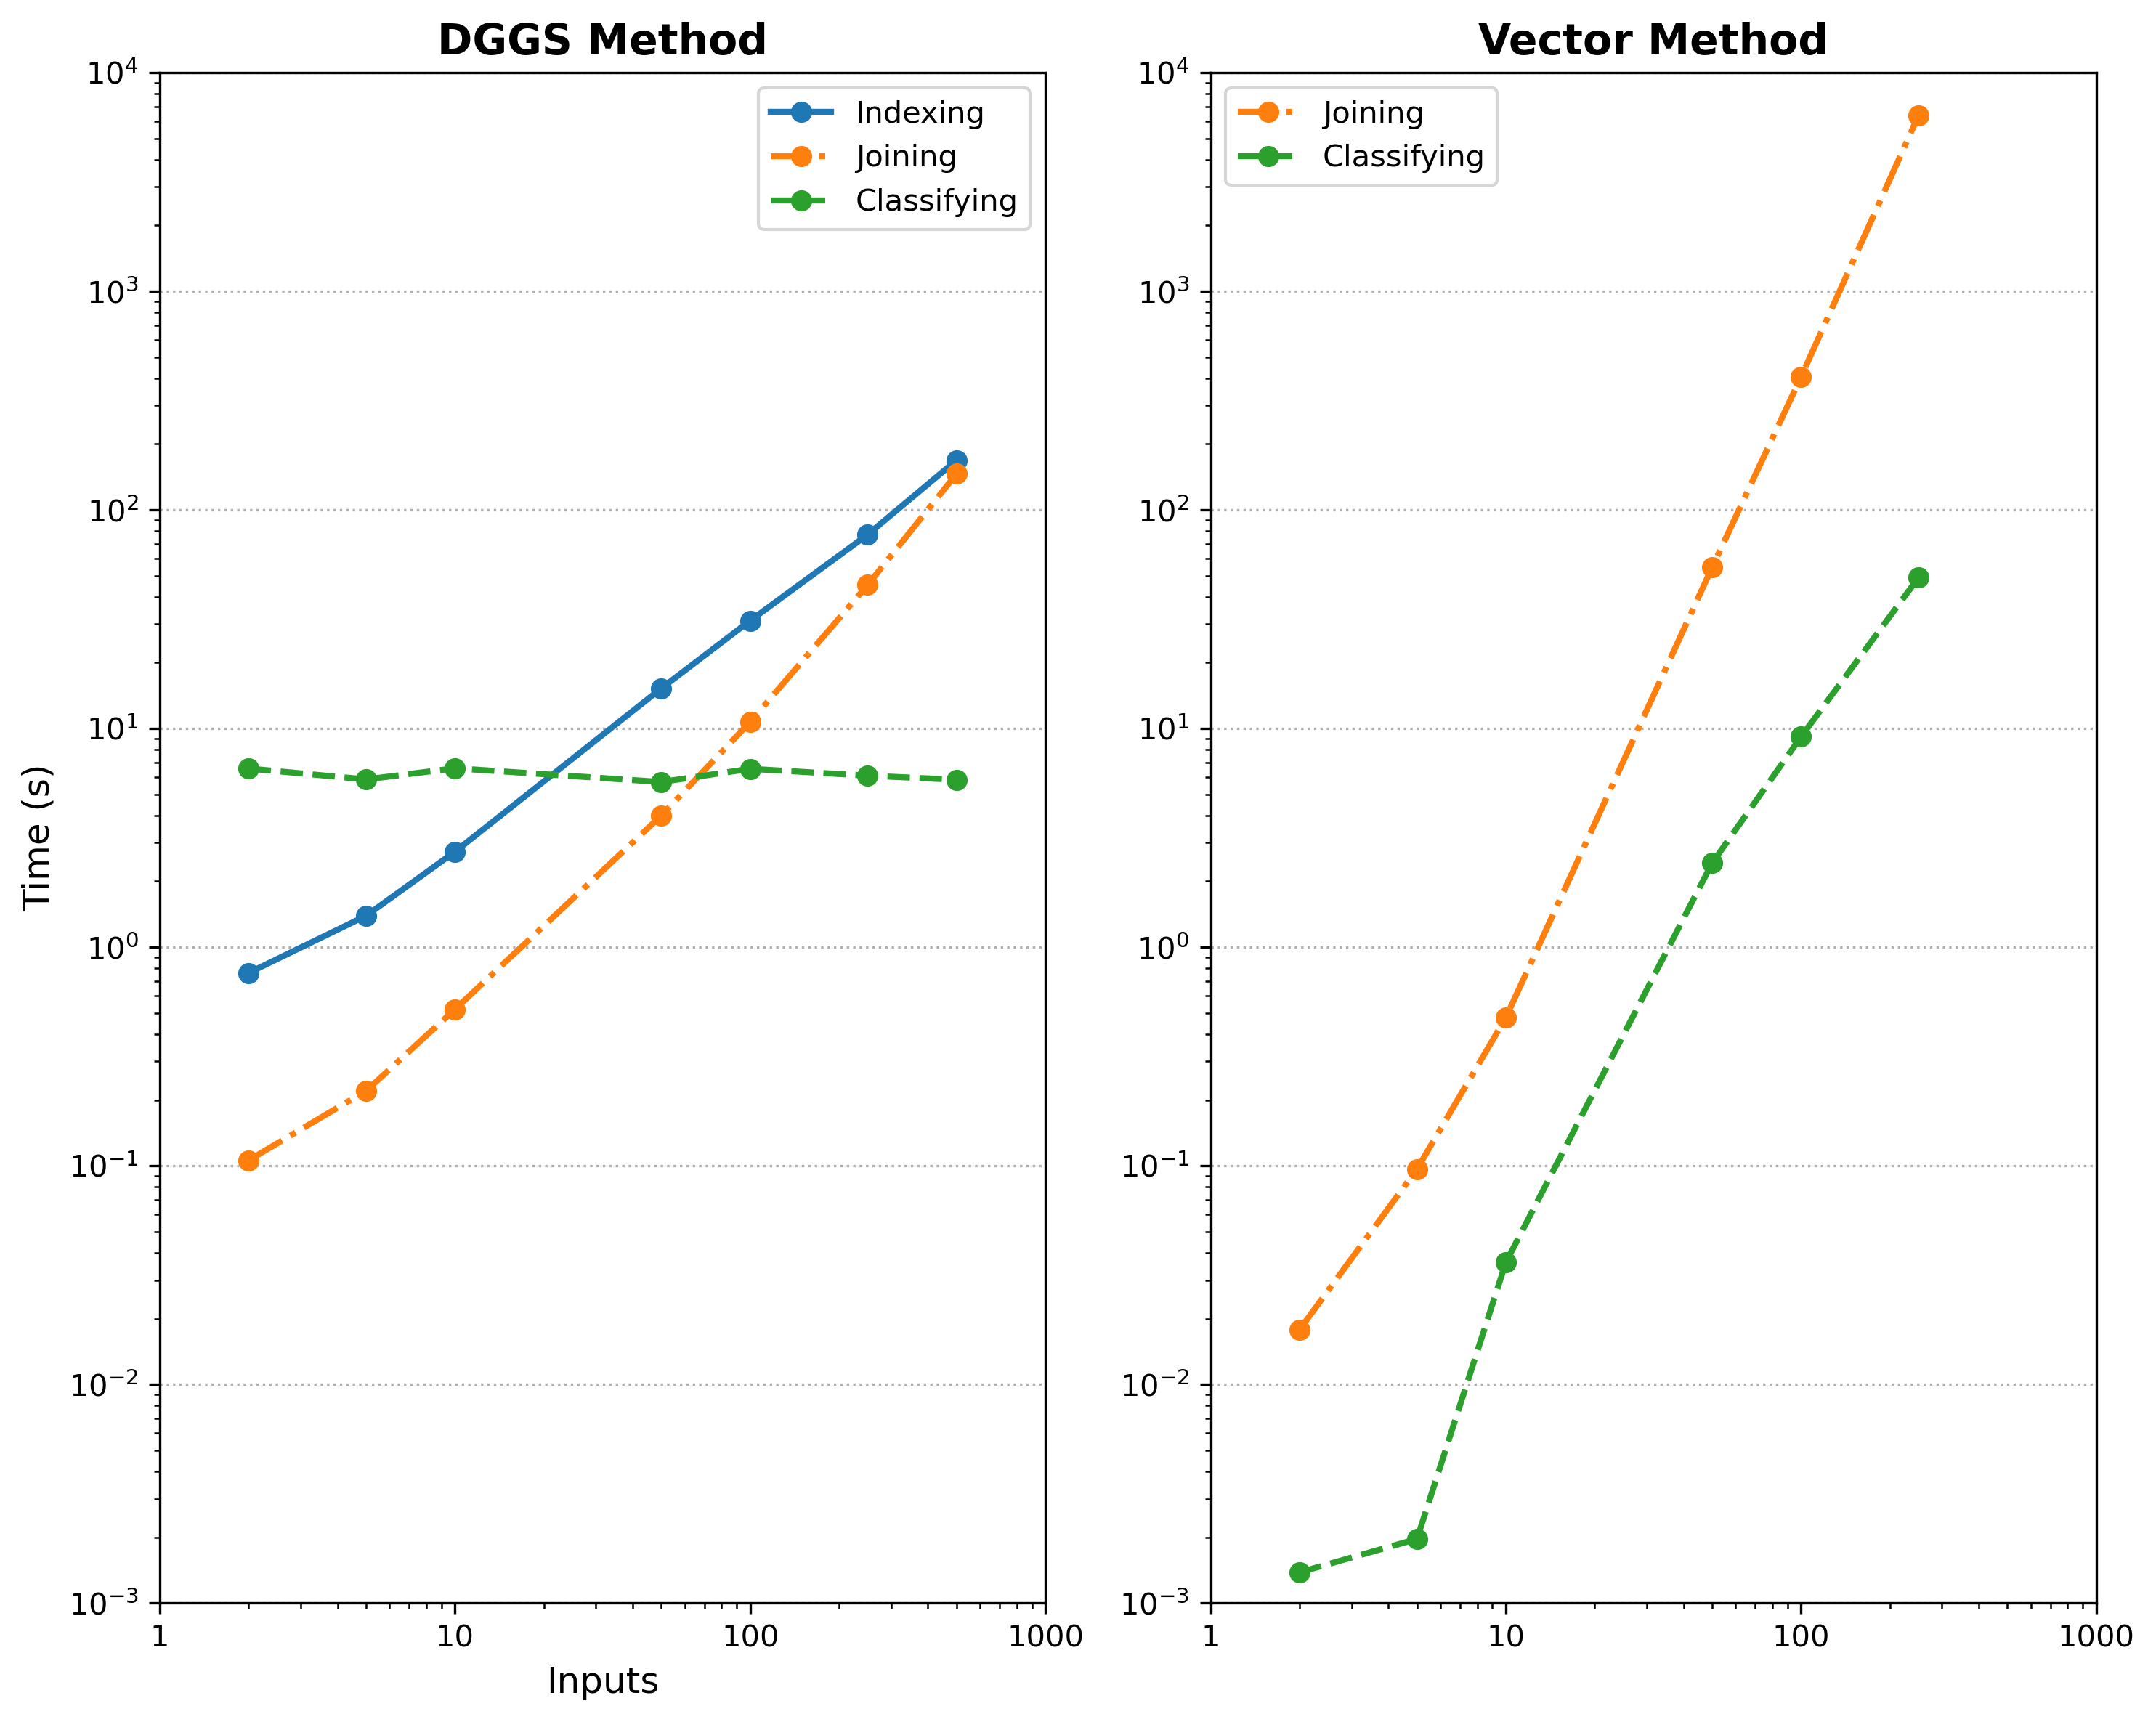
\includegraphics[width=0.85\linewidth]{images/vector-results.png}
    \caption{Vector benchmarking results. The charts are log-log plots with the number of vector input layers on the x-axis, and computational time in seconds on the y-axis. A \ac{DGGS} method for land-use mapping was several orders of magnitude more efficient than a na\"{i}ve vector overlay and map classification. Note that it was not possible to perform the vector method over 500 input layers on our benchmarking machine due to memory exhaustion.}
    \label{fig:BenchmarkVect}
\end{figure}

The results (Figure~\ref{fig:BenchmarkVect}) show that in the vector method the most expensive component is the initial spatial join (union). This appears to exhibit a power relationship as the number of inputs increases, to the point where it was not even feasible to perform the union with 500 inputs on our benchmarking computer. The application of the map classification to the vector layers was also a power function; this is because as the number of inputs increases, the number of small sliver polygons is likely to grow exponentially.

In contrast, the \ac{DGGS} method was several orders of magnitude more efficient overall, despite requiring the extra step of polyfilling. Classification itself was extremely efficient, and had barely no relationship to the number of input layers, due to the fixed discretisation of space whereby the number of zones to classify cannot grow with the number of input layers (it is related predictably to the chosen \ac{DGGS} resolution).

\subsubsection{Raster}

The model of discrete quantisation of space and aligned grids is common to \acp{DGGS} and raster analysis. The overhead of converting data to a \ac{DGGS} is similar to reprojecting and aligning raster data. Therefore we generated random raster data with random misalignment by jittering the origin point for each of 10,000 input files, by up to one pixel length in each dimension. Then later we include time spent warping these grids into alignment as part of the performance benchmark.

For the sake of realism, the raster data for the benchmark experiment was generated using a mid-point displacement \ac{NLM} \citep{etherington2015nlm}. 10,000 \ac{NLM} landscapes were generated, each 100 by 100 pixels. Discrete (ordinal) cases were generated by further transforming the synthetic landscapes into classes 1-10 with random weights \citep{etherington2015nlm}.

For each pixel (or \ac{DGGS} zone) in each input layer, there is a value between 0-1 (continuous) or 1-10 (discrete). The algorithm in each case aligns all inputs, and calculates the same eight Boolean values as in the vector case. Thereby there is $n\times8$ binary input layers in each case, which are then summed, and that value is considered to be the class label (for a possible $n\times8$ classes within a single output layer) where $n$ is the number of raster input datasets. Transformation from raster to \ac{DGGS} is performed by using rasterio\footnote{\url{https://rasterio.readthedocs.io}} to convert raster cells to coordinate pairs (cell centres), then converting these to H3 zone IDs, and then finally aggregating by zone IDs to account for multiple pixels potentially mapping to the same zone ID.

The results (Figure~\ref{fig:BenchmarkRast}) demonstrate equivalence between these techniques, which is expected as the conceptual similarity between how we use the \ac{DGGS} data model and the raster data model is much greater than in the vector case. Classification of \ac{DGGS} data is one order of magnitude faster than the raster method due to benefits accruing primarily to using a columnar data store (Apache Parquet) classified with a multi-threaded \ac{OLAP} query engine (Polars) which can easily apply map classification rules in parallel across all \ac{DGGS} zones \citep{polars}. The raster method could have been optimised further, so the difference is not considered significant; rather this demonstrates no expected performance penalty for using \ac{DGGS} over raster data models to perform equivalent work.

\begin{figure}[t]
    \centering
    % \resizebox{25pc}{!}{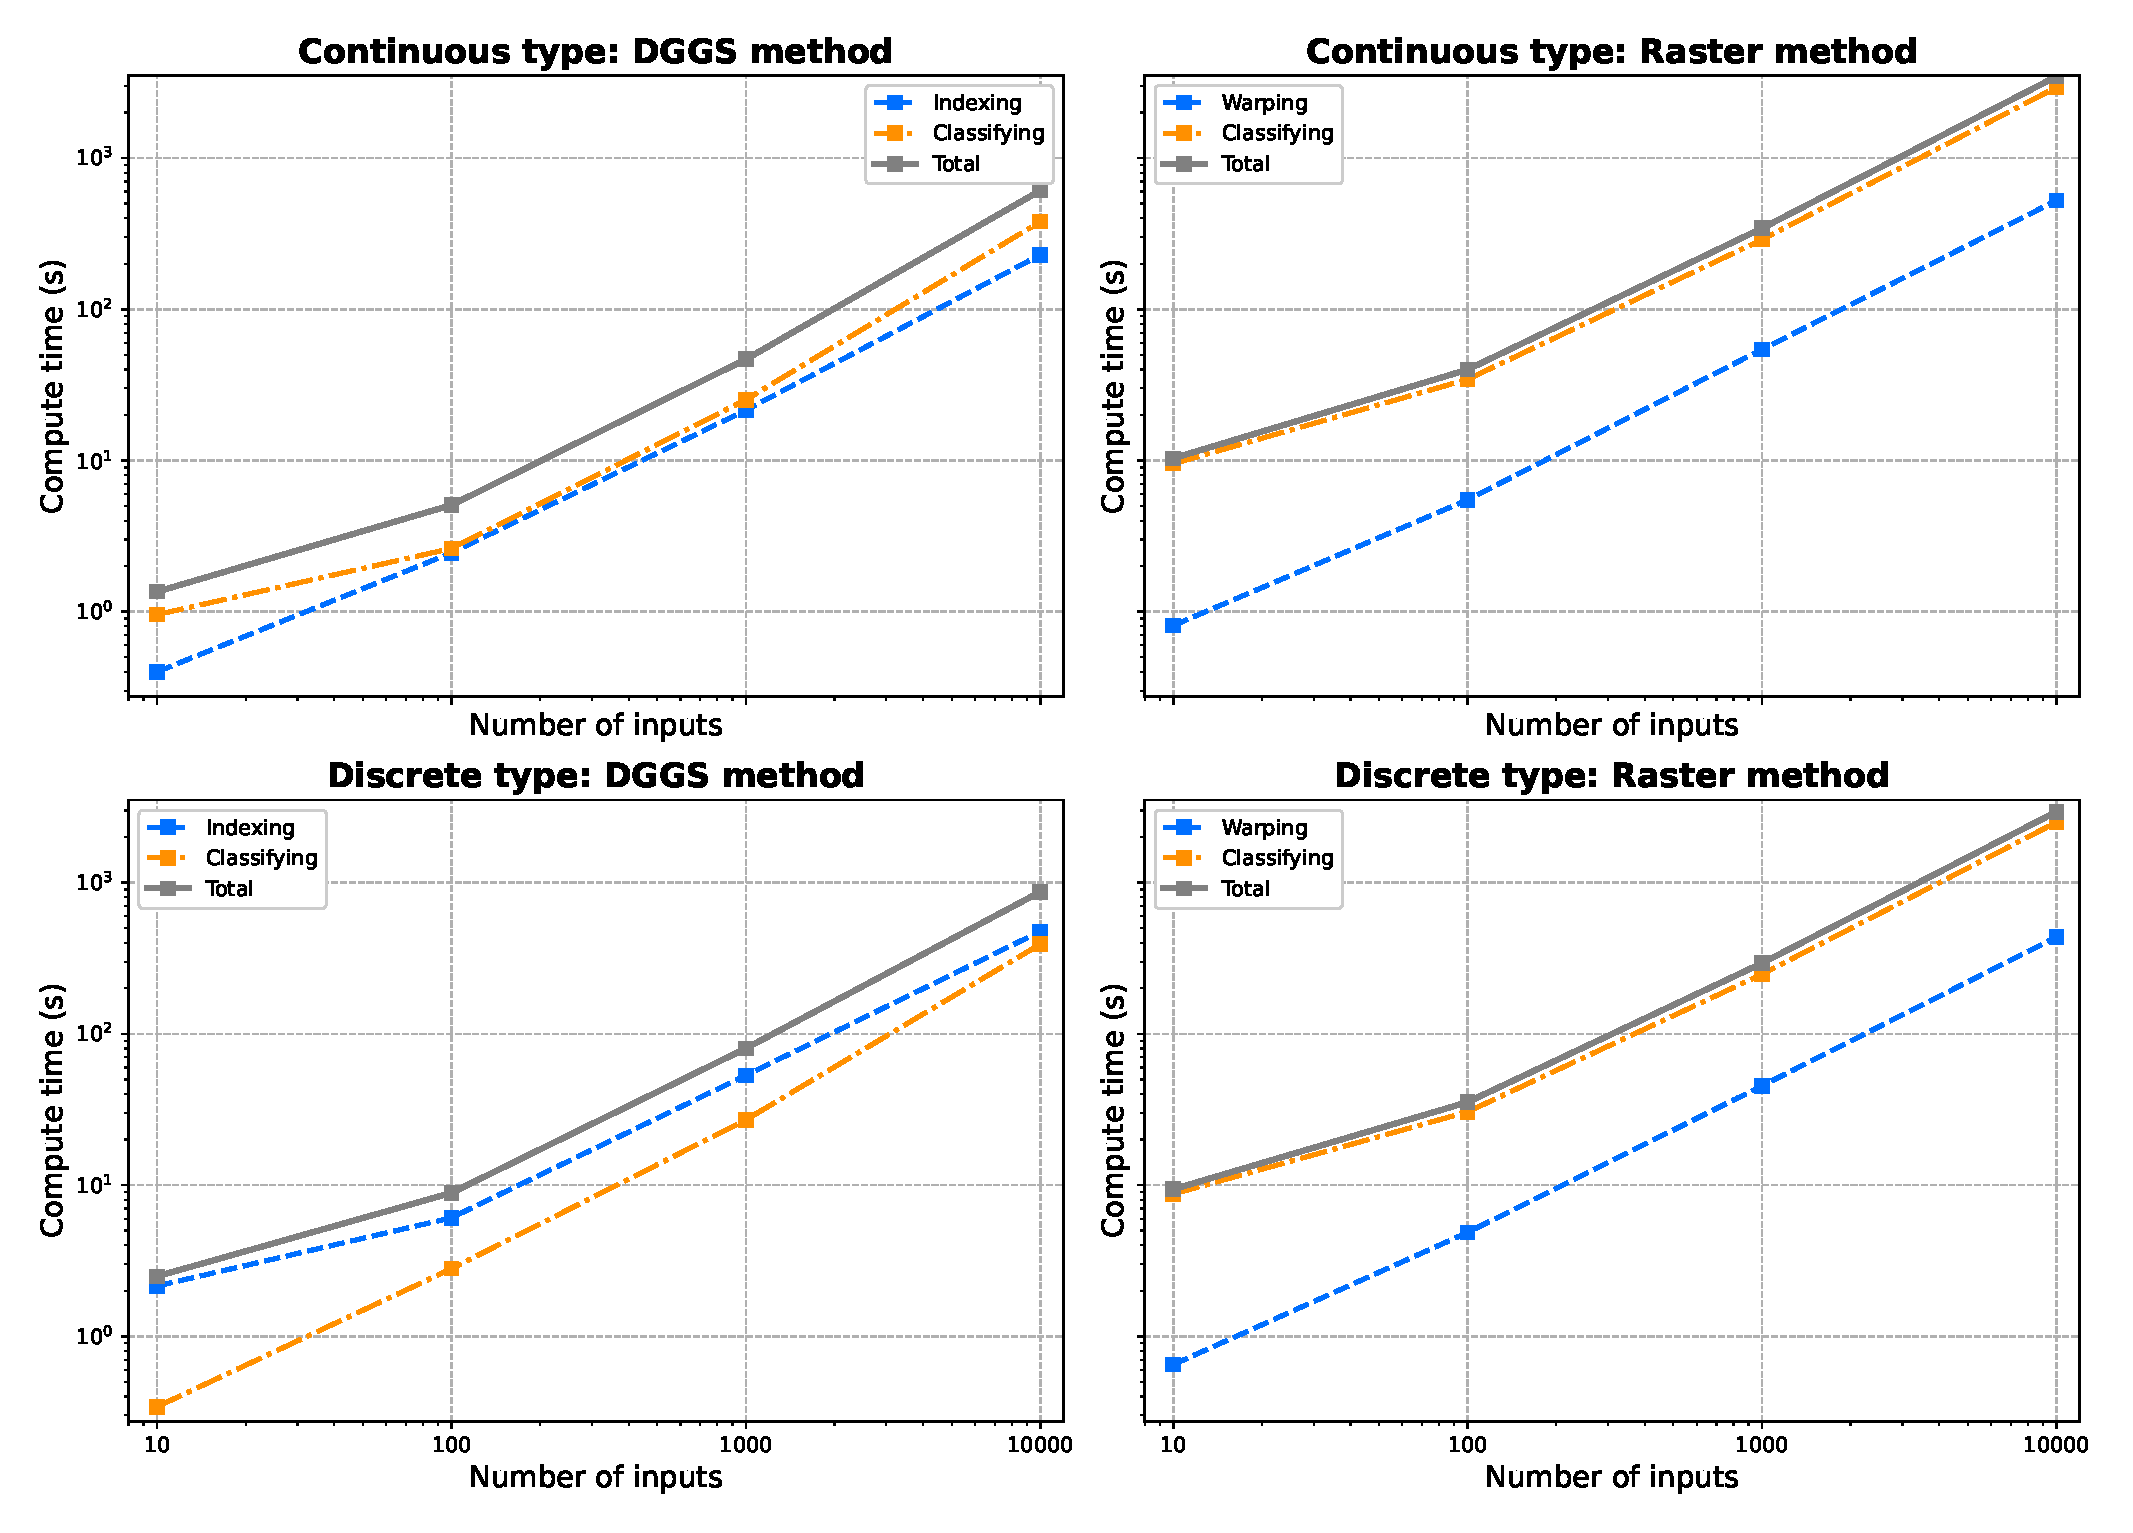
\includegraphics{images/raster-results.eps}}
    % 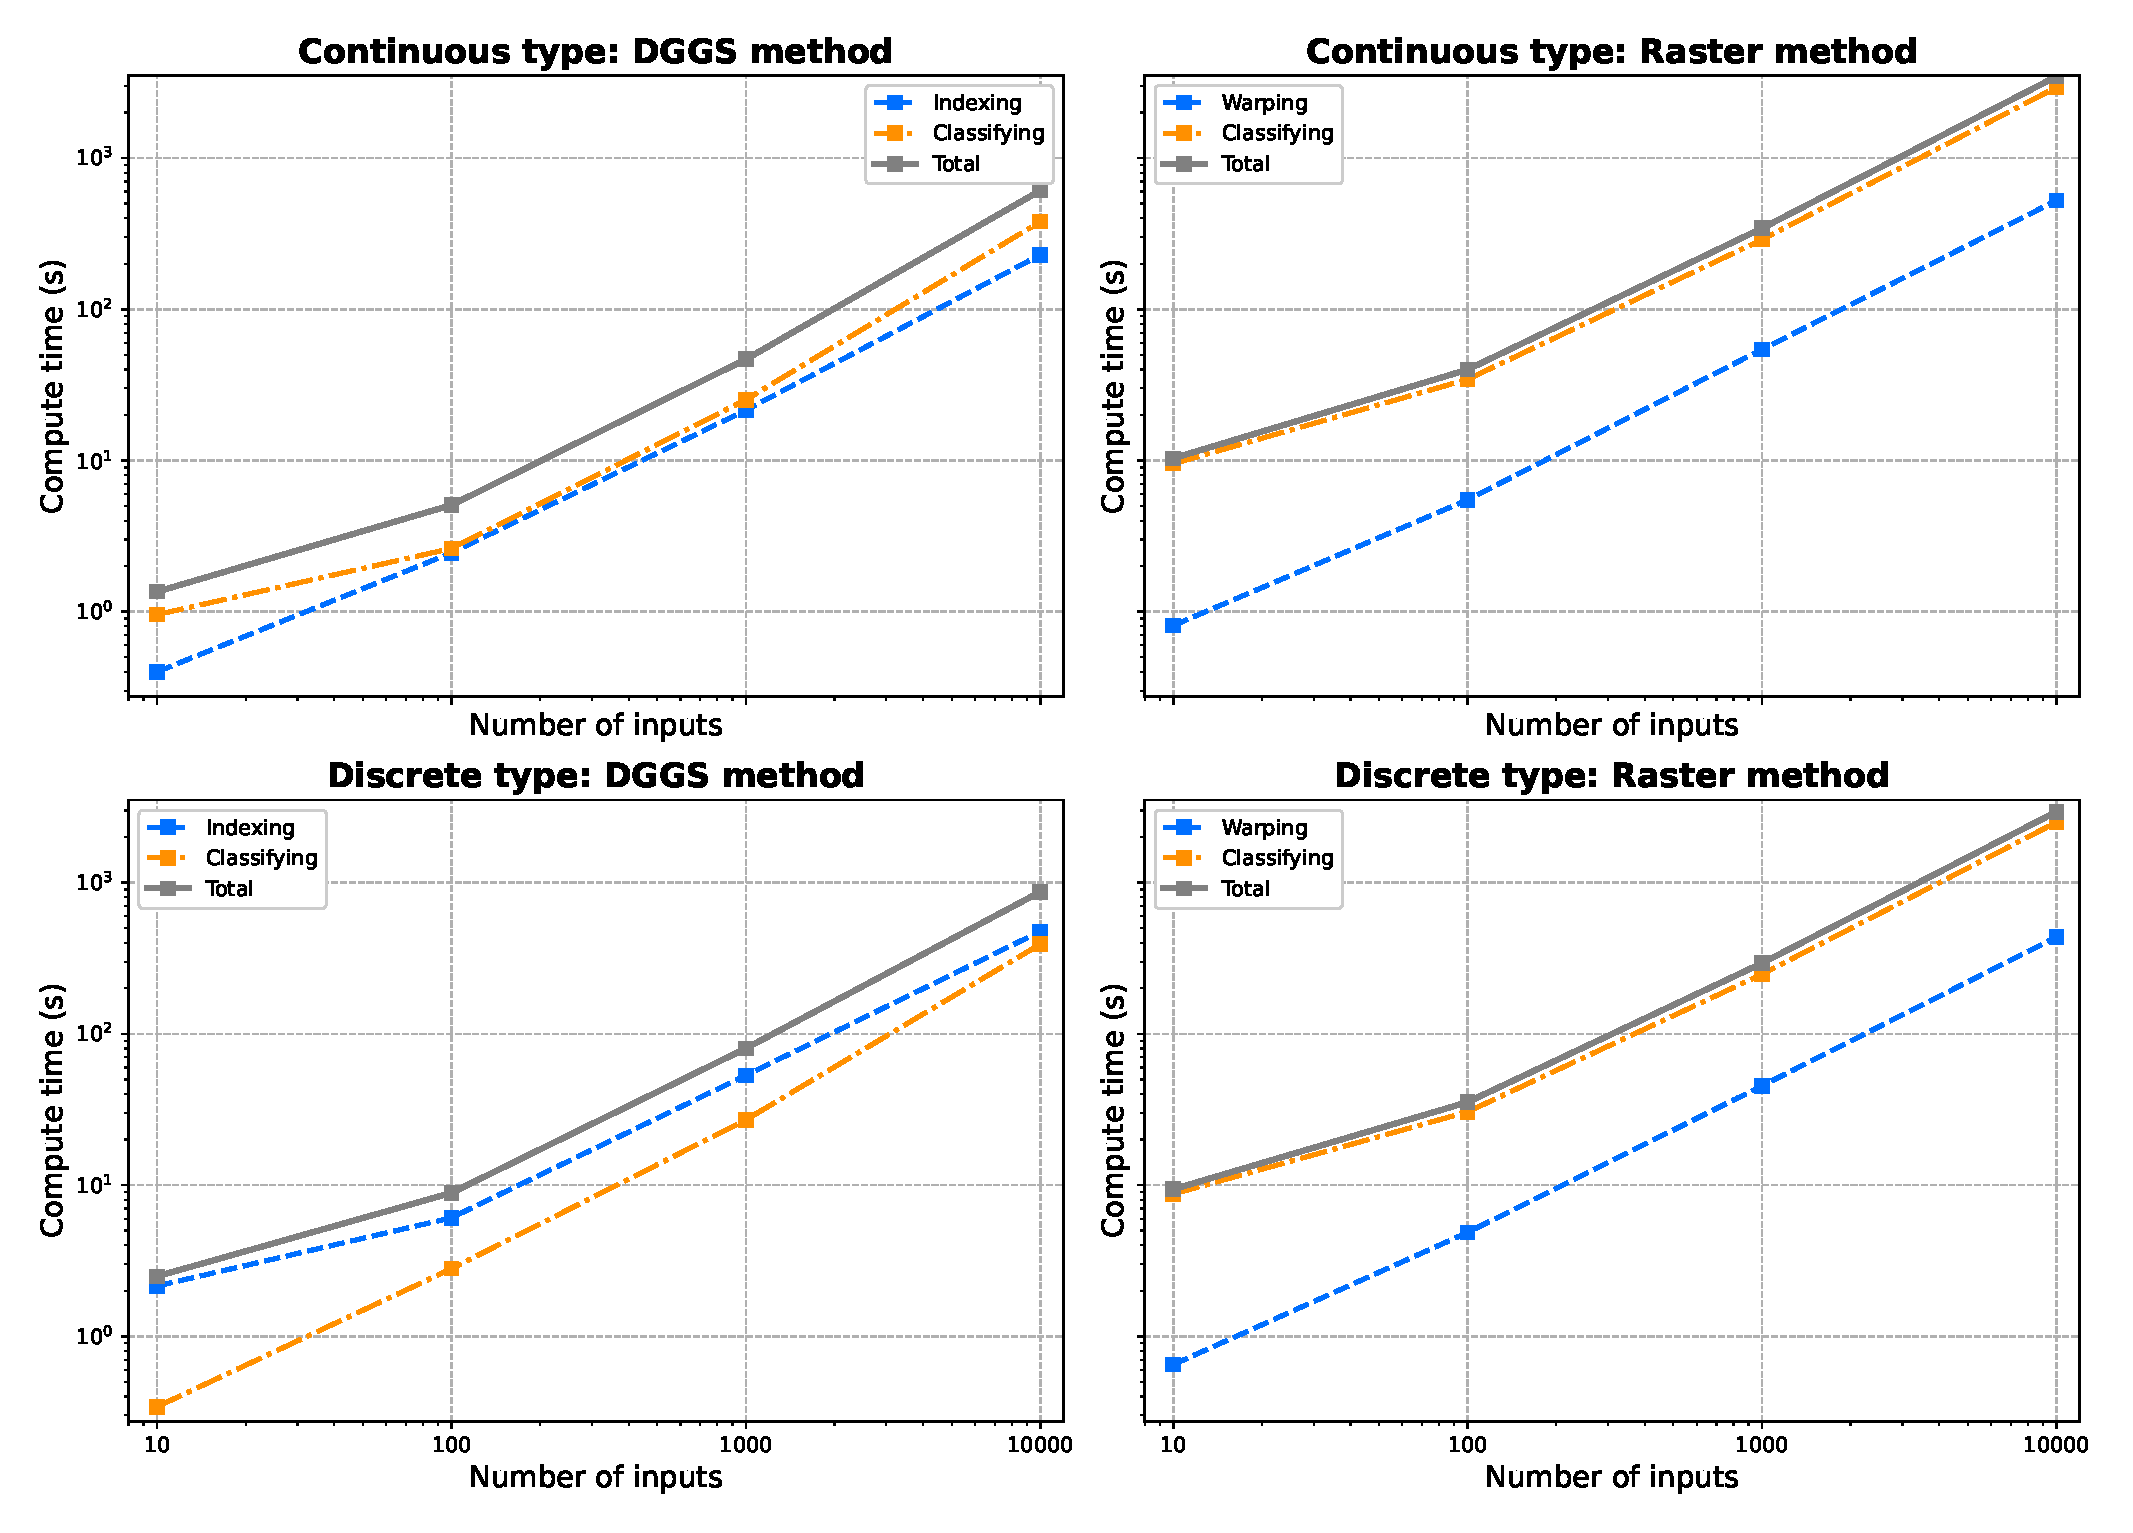
\includegraphics[width=0.85\linewidth]{images/raster-results.eps}
    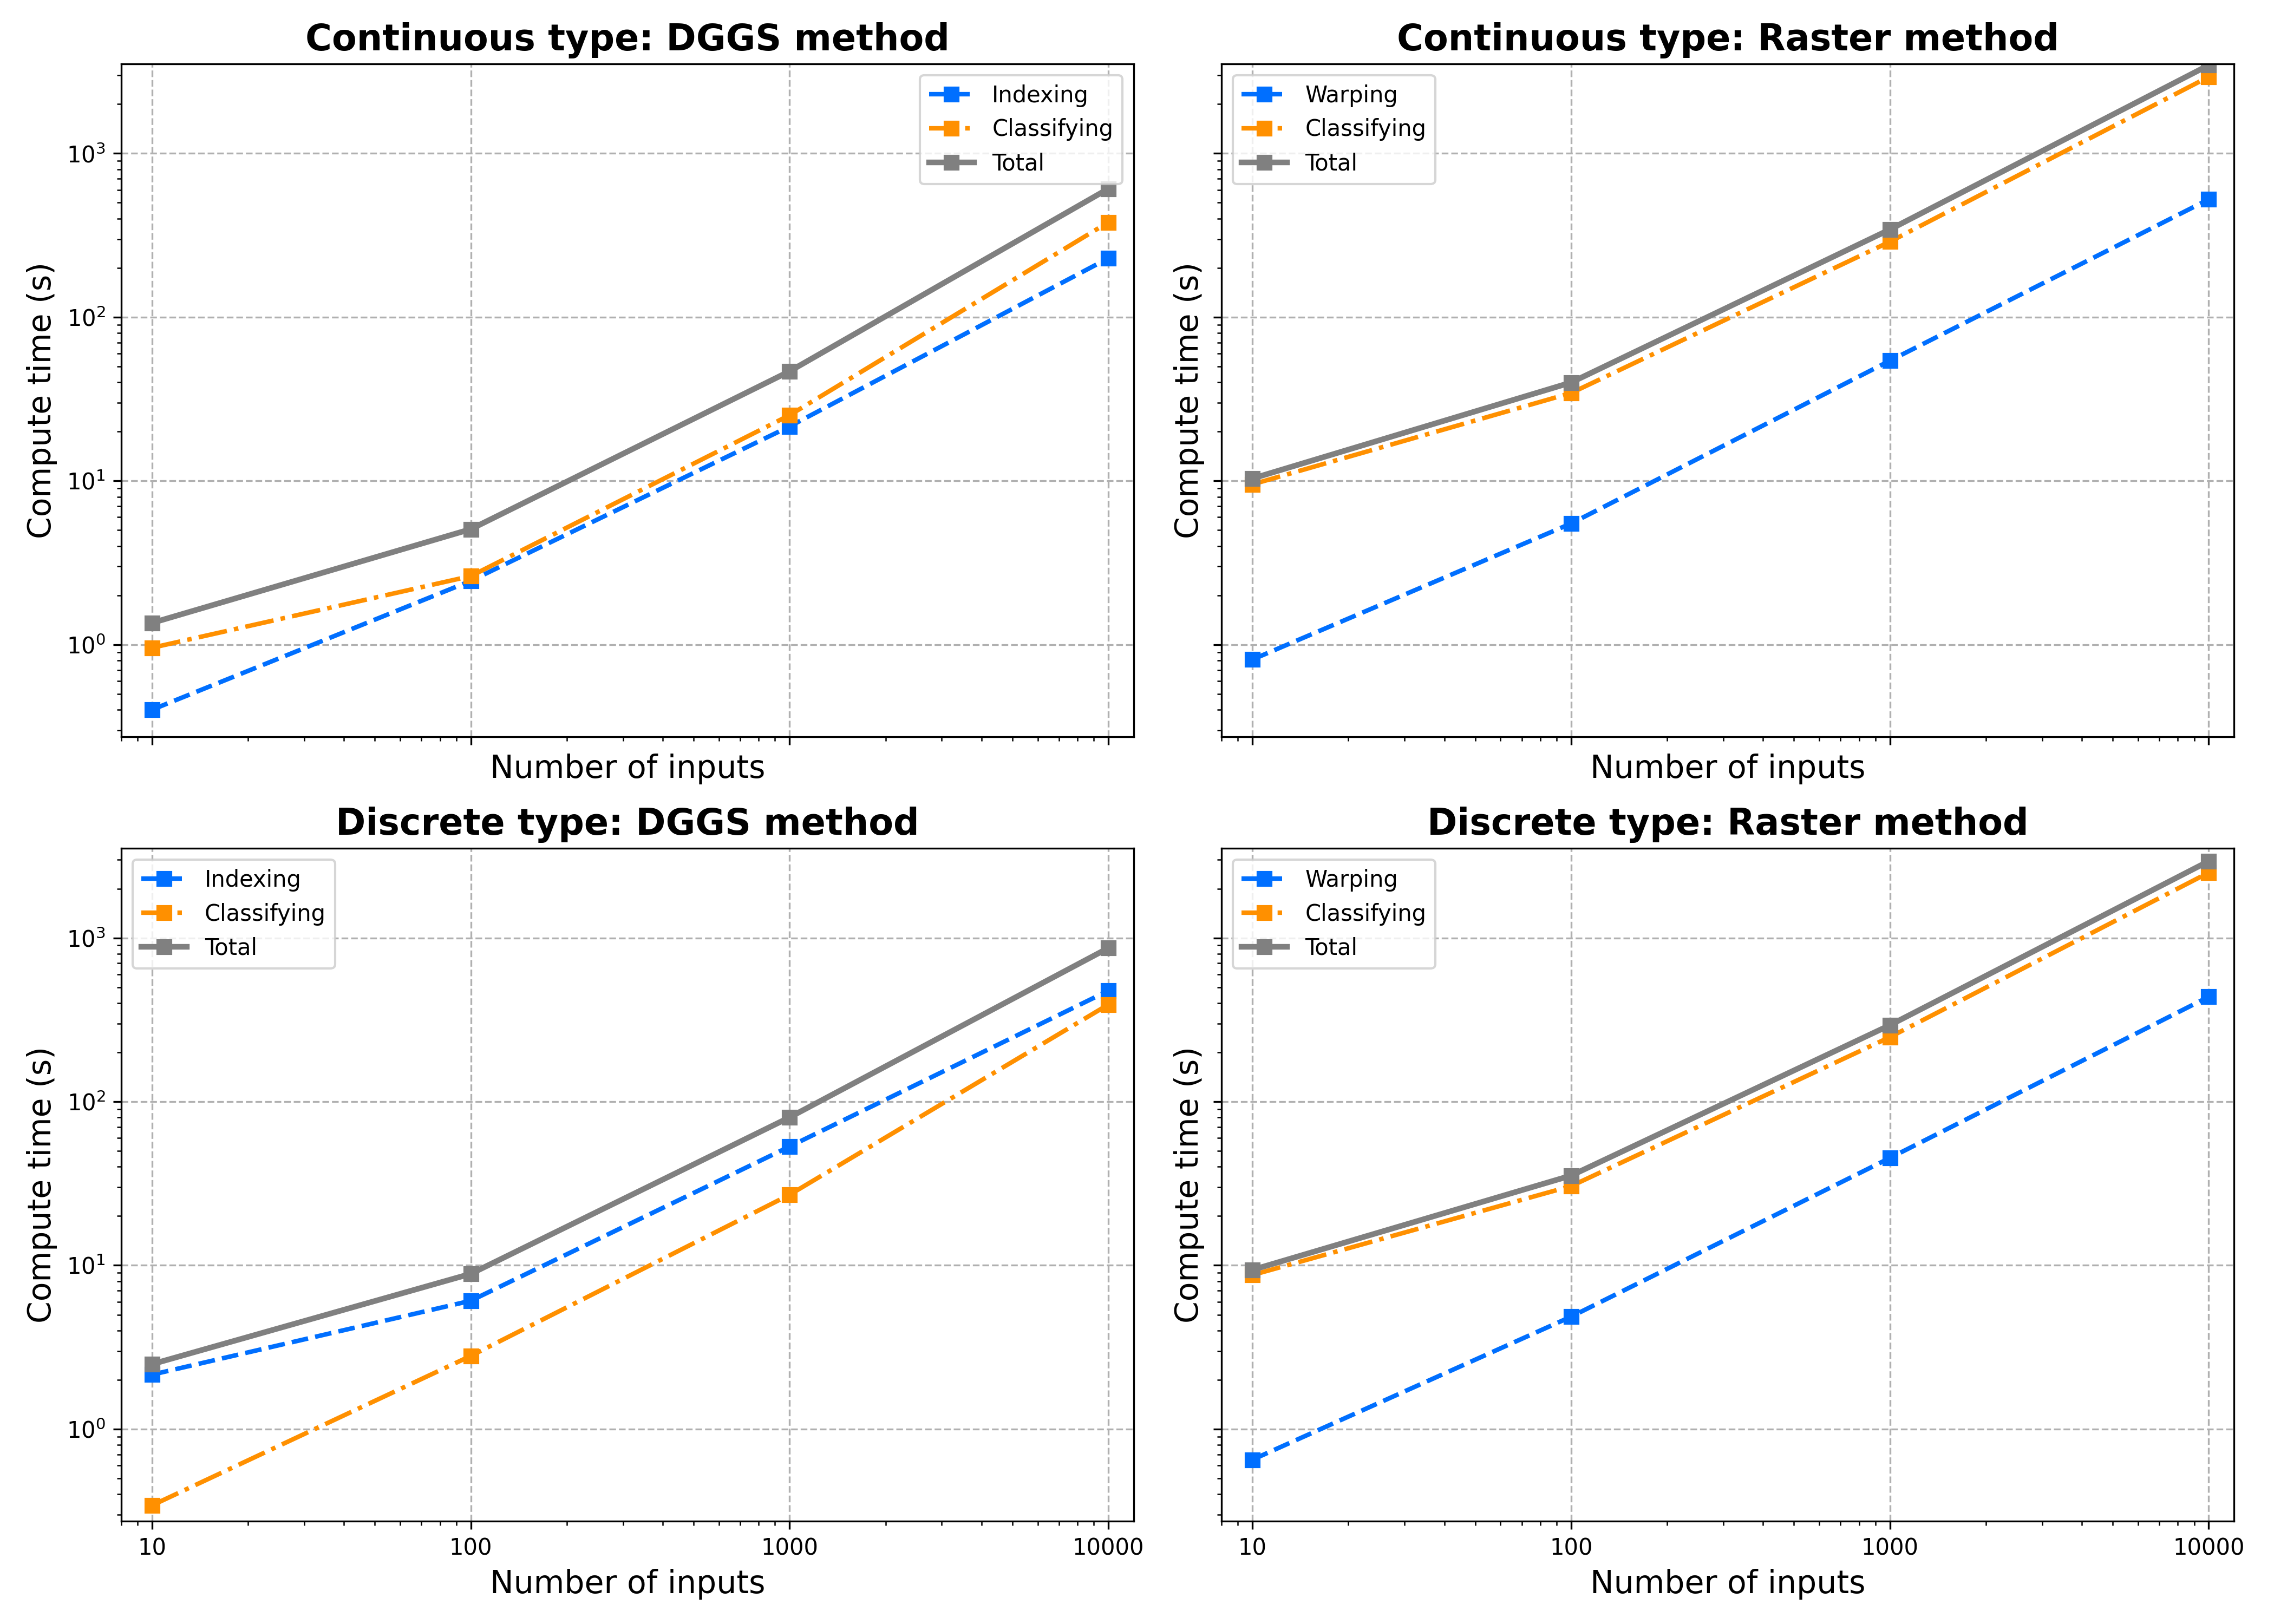
\includegraphics[width=0.85\linewidth]{images/raster-results.png}
    \caption{Raster input benchmarking results. The charts are log-log plots with the number of raster input layers on the x-axis, and computational time in seconds on the y-axis. These demonstrate roughly equivalent performance between raster and \ac{DGGS} methods of combination and deterministic map classification.}
    \label{fig:BenchmarkRast}
\end{figure}

\section{Discussion}

% - column-orientation doesn't suit algorithms or classification queries that need all columns, or if they need to compute pair-wise distance matrix
Much of the efficiency of organising geospatial information in a \ac{DGGS} is due to the query performance benefit of column-oriented data stores, such as Apache Parquet \citep{abadi2008column,ivanov2020impact}. The benefits of column-oriented data apply most effectively where queries are likely to only scan a subset of columns \citep{abadi2008query}. For a realistic land-use map classification rule, consider a query that requires three or four bands of a multiband sensor, and only a few census variables (of the hundreds that may be available). The execution of such a query could immediately avoid reading the majority of the available information when using a column-oriented data store \citep[pp.~232--238]{abadi2013design}. Yet this advantage does not apply when all available columns are necessary to the query (requires a complete scan), or where dynamic, pair-wise distance matrices are required (requires computing sort order dynamically, and reading data from multiple spatial partitions).

% - compression techniques only work well on sparse data types and factors, but not well on double-valued continuous data
One other relevant advantage of column-oriented data is in terms of benefits for data compression. If data is spatially partitioned (as it would most sensibly be with a \ac{DGGS} within a column-oriented data store), then adjacent data is very likely to be the same (the ``first law of geography'', \citet{tobler1970computer}) which makes compression more effective, using compression techniques such as bit-vector encoding, run-length encoding, or frame of reference values with delta coding \citep{abadi2013design}. Land-use classification is often effectively an exercise in re-classification of already classified information. Even information that is originally continuous can be pre-classified into bins or have thresholds applied to make it discrete before it is stored in a column-oriented format for later queries. Where this can be exploited, it should be; but where queries are likely to be dynamic, depend on high-precision continuous variables, and if data is highly spatially heterogenous, then the compression benefits will not be so apparent.

% - appends on column stores are expensive, so it is not ideal for streaming / changing data
Column-orientation is also effective for land-use mapping because such systems are often suitable for ``write-once, read-many'' use cases, where static input data is collected infrequently or only once, but queries are made more often (e.g. across multiple spatial partitions, for different map outputs, or in response to dynamic user input such as user-specific thresholds). Relative to a row-oriented data store, column-orientation incurs a penalty for appending new data, or deleting entire records \citep[p.~255]{abadi2013design}. Therefore for a land-use mapping process that makes use of streaming or dynamic data, the benefits would be more limited. However, common inputs such as satellite images, canopy height and terrain maps, census, and property records are not very dynamic, or else users only demand infrequent snapshots of land-use information.

In addition to the reasonably small performance benefit of \ac{DGGS} compared to raster, we note that a \ac{DGGS} analysis has two further benefits over a raster data model.

% Windowed reads
Firstly, computational efficiency is affected by raster block size, which is the preferred chunk size for efficient reads. For tiled rasters the block size is typically one tile. For scanline-oriented images this is usually one scanline. If component raster data do not share block sizes, performing a classification in parallel (i.e. in raster windows) is likely to be inefficient. In contrast, a \ac{DGGS} data model affords automatic and perfectly aligned spatial partitioning using zone parentage; a data model prepared for horizontal scaling.

% Text strings, array data types
Secondly, raster data types are typically limited to numeric types. Text categories can be encoded as numeric values, but rich text types and other complex types (such as array types) are difficult to encode and then to read when classifying. A \ac{DGGS} in any data storage and retrieval system can readily encode and read numerical, textual, and complex data types. Although there are raster formats that support the concept of \acp{RAT}, including the ERDAS IMAGINE File Format (IMG) and KEA files \citep{bunting2013}, \acp{RAT} remain largely unsupported in geospatial tools. This limits the utility of the raster data model in land-use mapping tasks specifically.

By using a \ac{DGGS} it is easier to retain the advantages of rich non-numeric data types that are harder to exploit in the raster data model. For example, a \ac{DGGS} model is trivially compatible with PostgreSQL, which provides two data types that are specifically designed for full text search.\footnote{\url{https://www.postgresql.org/docs/current/datatype-textsearch.html}} We have found this capability especially useful in land-use mapping where we discover that many datasets have unstructured text information, or information encoded in names such as ``Recreation Reserve'' or ``Recreational Park'', for which it is advantageous to have the capability to simply filter on the lemma form ``recreation''. Many other cases are more complicated than this; we found text search types to be extremely valuable, required no adjustment to the workflow, could be adapted flexibly, and, due to PostgreSQL's \texttt{tsvector} type, were already optimised. With a raster workflow, preserving the information from text, array, blob or other non-numeric datatypes is difficult. A \ac{DGGS} workflow therefore has the spatial alignment benefits of a raster workflow, but fewer downsides.

The downsides of adopting a \ac{DGGS} data model include some apparent fidelity vis-\`{a}-vis the vector data model, immaturity and lack of optimisation for certain tools, the unfamiliarity of the data model to end users, problematic use of \acp{DGGS} with unequal-area cells, difficulty finding an appropriate \ac{DGGS} (e.g. one with a resolution with cells close to the native raster resolution), and lack of integration with existing geospatial tools such as PROJ \citep{thompson2022ease}. These are not all major downsides. For instance, the apparent loss of fidelity to vector data may not be significant if the application of the \ac{DGGS} can tolerate some level of error, or it may indeed be more realistic if additional precision beyond some threshold is really false precision; \acp{DGGS} such as rHEALPix do have PROJ codes; and familiarity with \ac{DGGS} ideas is progressing with developers and end-users.

\section{Conclusion}

Our experience and benchmarking results for land-use assignment demonstrate the utility of \acp{DGGS} for land classification generally, but land-use assignment in particular. Land-use assignment has a strong requirement for the integration of discrete and continuous raster data with ancillary vector data. As the classification becomes more complex and requires greater inputs, the need for efficient scaling becomes more pressing. A \ac{DGGS}, as a space-partitioned data structure, directly provides a means to horizontal scalability in \ac{GIS} workflows. Such workflows obviate the distinction between raster and vector data models, are efficient enough to enable iterative development of land-use assignment rules, and are readily compatible with modern data science principles such as the use of dataframes, array databases, and row-oriented data stores.

\clearpage

%TC:ignore
\section*{Disclosure statement}

The authors report there are no competing interests to declare.

\section*{Funding details}

This research was supported by Strategic Science Investment Funding (SSIF) for Crown Research Institutes from the New Zealand Ministry of Business, Innovation and Employment's Science and Innovation Group contract No. C09X1704.

\section*{Data availability statement}
The code written to generate the benchmark cases, and to measure the performance of the test cases, is available at \url{https://github.com/manaakiwhenua/dggsBenchmarks/releases/tag/v1.0}. The thousands of benchmark files are not provided, but can be regenerated: the data is synthetic and the scripts seed random number generators to produce deterministic outputs.

\section*{Notes on contributors}

\begin{wrapfigure}[10]{l}{0.3\textwidth}
\centering

\includegraphics[width=0.3\textwidth]{images/richard}
\end{wrapfigure}
\textbf{Richard Law} is a Geospatial Analyst at Manaaki Whenua -- Landcare Research, located in Palmerston North, New Zealand. He holds a Master of \ac{GISc}, which he completed in 2015 at Victoria University. Additionally, he earned a Bachelor of Science in Geography and Public Policy from Victoria University in 2013. In his role at Manaaki Whenua, Richard leverages his expertise in \ac{GIS} to support research projects that aim to manage and enhance New Zealand's land resources.\\

\begin{wrapfigure}[7]{l}{0.3\textwidth}
\centering

\includegraphics[width=0.3\textwidth]{images/james.jpg}
\end{wrapfigure}
\textbf{James Ardo} is a Geospatial Analyst at Manaaki Whenua -- Landcare Research in Palmerston North, New Zealand. He holds a Master of Science degree from Massey University, which he completed in 2022. His academic background and professional focus encompass a range of earth sciences, with particular interests in volcanology, sedimentology, and \ac{GIS}.\\

\clearpage


\bibliographystyle{apacite}
\bibliography{references}

%TC:endignore
\end{document}
